\hyphenation{se-para-tion}
\hyphenation{theo-re-ti-cal}
\hyphenation{handed-ness}
%______________________ Theory ______________________
\chapter{Theoretical approach}
\label{ch:theory}

%______________________ INTRODUCCION ______________________
\section{Introduction}
\label{secc:Intro_th}

The physical description of the universe is a challenge that physicists have faced by making theories that refine existing principles and proposing new ones in an attempt to embrace emerging facts and phenomena.
%% By early 1800's, there were separate theories describing electric and magnetic phenomena, gravitational force and light. The invention of the electric battery by Alessandro Volta in 1800, the discovery of the magnetic effects of the electric current by Oersted and Ampere (1820), and the generation of electric current using changing magnetic fields by Faraday (1831) represent the first steps in the way to create a unified theory describing electric and magnetic phenomena, the theory of electromagnetism \cite{griffiths}.\\

%% The unification was carried out by James Clerk Maxwell who was able to merge electricity and magnetism in a set of 20 equations known as \ti{general equations of the electromagnetic field,} relating the observables that describe the experimental laws of the electromagnetism. By combining these equations, Maxwell found a wave equation and propose the existence of the \ti{electromagnetic waves.} The predicted propagation speed of the electromagnetic waves turned out to be the same as the speed of light, therefore, the natural conclusion was that light is an electromagnetic wave\cite{maxwell}.

%% %By 1900, waves were considered a perturbation of a material medium which in the case of the electromagnetic waves was identified as the \textit{``Luminiferous Ether}}.
%% By 1900, Max Planck came out with the idea that radiation is quantized\cite{planck} and Albert Einstein in 1905 made use of that hypothesis to propose the existence of the light quantum, the \textit{``photon}}, in order to explain the photoelectric effect\cite{photoeffect}. The well-known quantum revolution in physics started and the idea of particle-wave duality of photons as a natural behavior was developed and later extended to electrons and to all kind of particles in nature. The development of a quantum theory allowed to predict a set of non-common sense effects like the quantum tunneling and quantum entanglement, however, quantum theory was separated from the recently unified electromagnetism.\\

%% In 1905, Einstein also published two more papers; one aimed to describe his statistical molecular theory of liquids and how it can be used to describe Brownian motion\cite{brownian}. At that time the existence of the atoms and molecules were not fully demonstrated but Einstein's theory provided an explanation as well as predictions based on the their existence. Jean Perrin in 1908 conducted experiments that confirmed Einstein's predictions. The other paper described the relationship between space and time \cite{relativity}, unifying the notion of space and time into one entity known as \textit{spacetime} that treats space and time at the same level and then discards the absoluteness of time. The new theory known as special relativity, supersedes the Galilean relativity principle and postulates exceptional effects like the time dilation, length contraction and mass-energy equivalence through the most famous formula in physics\cite{energy}
%% \beqn
%% E=mc^2.
%% \eeqn
%% Generalization of the special relativity was presented in 1916 and includes a generalization of Newton's law of universal gravitation, becoming a unified description of gravity as a geometric property of space and time. Einstein's predictions include the existence of black holes and the recently observed \textit{gravitational waves}\cite{ligo}.  

At the end of 1940s Julian Schwinger\cite{schwinger} and Richard P. Feynman\cite{feynman}, based on the work of Sin-Itiro Tomonaga\cite{tomonaga}, developed an electromagnetic theory consistent with special relativity and quantum mechanics that describes how matter and light interact; the so-called \ti{quantum electrodynamics} (QED) was born.% Despite the incredible success of general relativity in describing the macroworld where gravity dominates and quantum mechanics in describing the microworld where other forces dominates, a self-consistent theory of quantum gravity is not yet available.

QED has become the guide in the development of theories that describe the universe. It was the first example of a quantum field theory (QFT), which is the theoretical framework for building quantum mechanical models that describes particles and their interactions. QFT is composed of a set of mathematical tools that combines classical fields, special relativity and quantum mechanics, while keeping the quantum point particles and locality ideas.

This chapter gives an overview of the standard model of particle physics, starting with a description of the particles and interactions that compose it, followed by a description of the electroweak interaction, the Higgs boson and the associated production of Higgs boson and a single top quark ($tH$). The description contained in this chapter is based on References \cite{griffiths, mandl, halzen}.  % The last section gives an overview of the CP-mixing implications in tH processes.      

%______________________ SM  ______________________
\section{Standard model of particle physics}
\label{secc:SM}

Particle physics at the fundamental level is modeled in terms of a collection of interacting particles and fields in a theory known as the \ti{standard model of particle physics (SM)}. The full picture of the SM is composed of three fields\footnote{The formal and complete treatment of the SM is out of the scope of this document, however a plenty of textbooks describing it at several levels are available in the literature. The treatment in References \cite{mandl,halzen} is quite comprehensive and detailed. Note that gravitational field is not included in the standard model formulation} whose excitations are interpreted as particles called mediators or force-carriers, a set of fields whose excitations are interpreted as elementary particles interacting through the exchange of those mediators, and a field that gives the mass to elementary particles. Figure \ref{sm} shows the scheme of the SM particles' organization. In addition, for each of the particles in the scheme there exits an antiparticle with the same mass and opposite quantum numbers. The existence of antiparticles is a prediction of the relativistic quantum mechanics from the solution of the Dirac equation for which a negative energy solution is also possible. In some cases a particle is its own anti-particle, like photon or Higgs boson.

\begin{figure}[h!]
  \centering
  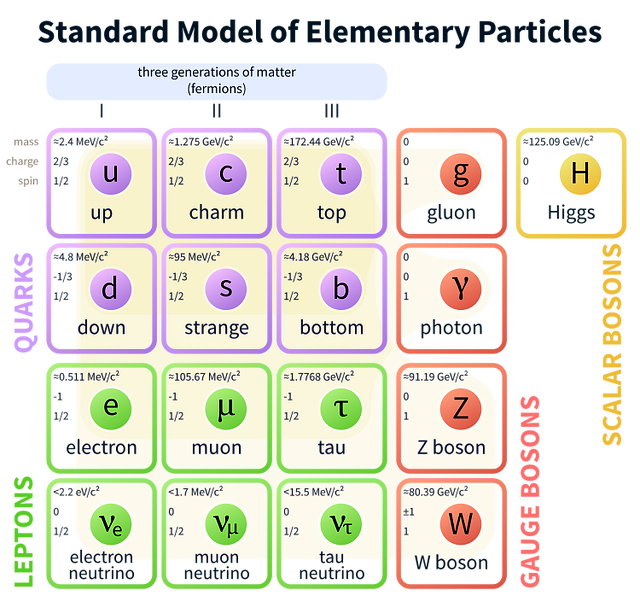
\includegraphics[scale=0.4]{sm}
  \caption[Standard Model of particle physics.]{Schematic representation of the Standard Model of particle physics. The SM is a theoretical model intended to describe three of the four fundamental forces of the universe in terms of a set of particles and their interactions. \cite{smpicture}.}
  \label{sm}
\end{figure}

The mathematical formulation of the SM is based on group theory and the use of Noether's theorem\cite{noether} which states that for a physical system modeled by a Lagrangian that is invariant under a group of transformations a conservation law is expected. For instance, a system described by a time-independent Lagrangian is invariant (symmetric) under time changes (transformations) with the total energy conservation law as the expected conservation law. In QED, the charge operator (Q) is the generator of the U(1) symmetry which according to the Noether's theorem means that there is a conserved quantity; this conserved quantity is the electric charge and thus the law conservation of electric charge is established.

In the SM, the symmetry group $SU(3)_C\otimes SU(2)_L\otimes U(1)_Y$ describes three of the four fundamental interactions in nature (see Section \ref{fund_inter}): strong interaction (SI), weak interaction (WI) and electromagnetic interactions (EI) in terms of symmetries associated to physical quantities:
\begin{itemize}
\item Strong: $SU(3)_C$ associated to color charge
\item Weak: $SU(2)_L$ associated to weak isospin and chirality
\item Electromagnetic: $U(1)_Y$ associated to weak hypercharge and electric charge
\end{itemize}

It will be shown that the electromagnetic and weak interactions are combined in the so-called electroweak interaction where chirality, hypercharge, weak isospin and electric charge are the central concepts.

\subsection{Fermions}\label{fermions}

The basic constituents of the ordinary matter at the lowest level, which form the set of elementary particles in the SM formulation, are quarks and leptons. All of them have spin 1/2, therefore they are classified as fermions since they obey Fermi-Dirac statistics. There are six \ti{flavors} of quarks and three of leptons organized in three generations, or families, as shown in Table \ref{flav_gen}.\\
 
\begin{center}
\begin{table}[h!]
\centering
\footnotesize
\begin{tabular}{ccccc} \hline
                         &         & \multicolumn{3}{c}{Generation}                                                           \\ \hline
                         &Type     & 1st                          & 2nd                        & 3rd                          \\ \hline
\multirow{2}{*}{Leptons} &Charged  & Electron (e)                 & Moun($\mu$)                & Tau ($\tau$)                 \\%\hline
                         &Neutral  & Electron neutrino ($\nu_e$)  & Muon neutrino ($\nu_{\mu}$) & Tau neutrino ($\nu_{\tau}$) \\\hline
\multirow{2}{*}{Quarks}  &Up-type  & Up (u)                       & Charm (c)                & Top (t)                        \\%\hline
                         &Down-type& Down (d)                     & Strange (s)              & Bottom (b)                     \\\hline
\end{tabular}
\caption[Fermions of the SM.]{Fermions of the SM. There are six flavors of quarks and three of leptons, organized in three generations, or families, composed of two pairs of closely related particles. The close relationship is motivated by the fact that each pair of particles is a member of an $SU(2)_L$ doublet that has an associated invariance under isospin transformations. WI between leptons is limited to the members of the same generation; WI between quarks is not limited but greatly favored, to same generation members. }\label{flav_gen}
\end{table}
\end{center}

There is a mass hierarchy between generations (see Table \ref{f_masses}), where the higher generation particles decays to the lower one, which can explain why the ordinary matter is made of particles from the first generation. In the SM, neutrinos are modeled as massless particles so they are not subject to this mass hierarchy; however, today it is known that neutrinos are massive so the hierarchy could be restated. The reason behind this mass hierarchy is one of the most important open questions in particle physics, and it becomes more puzzling when noticing that the mass difference between first and second generation fermions is small compared to the mass difference with respect to the third generation.
\begin{center}
\begin{table}[h]
\centering
\footnotesize
\begin{tabular}{lclc} \hline
Lepton    & Mass (MeV/c$^2$) & Quark  & Mass (MeV/c$^2$)       \\ \hline
e         & 0.51             & u      & $ 2.2$             \\ %\hline
$\mu$     & 105.65           & c      & $ 1.28\times 10^3$ \\ %\hline
$\tau$    & 1776.86          & t      & $ 173.1\times 10^3$\\ %\hline
$\nu_e$   & Unknown          & d      & $ 4.7$             \\ %\hline
$\nu_\mu$ & Unknown          & s      & $ 96$              \\ %\hline
$\tau_\mu$& Unknown          & b      & $ 4.18\times 10^3$ \\ \hline
\end{tabular}
\caption[Fermion masses.]{Fermion masses\cite{pdg}. Generations differ by mass in a way that has been interpreted as a mass hierarchy. Approximate values with no uncertainties are used, for comparison purpose.}\label{f_masses}
\end{table}
\end{center}

Usually, the second and third generation fermions are produced in high energy processes, like the ones recreated in particle accelerators.         

\subsubsection{Leptons}

A lepton is an elementary particle that is not subject to the SI. As seen in Table \ref{flav_gen}, there are two types of leptons, the charged ones (electron, muon and tau) and the neutral ones (the three neutrinos). The electric charge (Q) is the property that gives leptons the ability to participate in the EI. From the classical point of view, Q plays a central role determining, among others, the strength of the electric field through which the electromagnetic force is exerted. It is clear that neutrinos are not affected by EI because they don't carry electric charge.

Another feature of the leptons that is fundamental in the mathematical description of the SM is the chirality, which is closely related to spin and helicity. Helicity defines the handedness of a particle by relating its spin and momentum such that if they are parallel then the particle is right-handed; if spin and momentum are antiparallel the particle is said to be left-handed. The study of parity conservation (or violation) in $\beta$-decay has shown that only left-handed electrons/neutrinos or right-handed positrons/anti-neutrinos are created\cite{goldhaber}; the inclusion of that feature in the theory was achieved by using projection operators for helicity, however, helicity is frame dependent for massive particles which makes it not Lorentz invariant and then another related attribute has to be used: \textit{chirality}.

Chirality is a purely quantum attribute which makes it not so easy to describe in graphical terms but it defines how the wave function of a particle transforms under certain rotations. As with helicity, there are two chiral states, left-handed chiral (L) and right-handed chiral (R). In the highly relativistic limit where $E\approx p \gg m$ helicity and chirality converge, becoming exactly the same for massless particles.

In the following, when referring to left-handed (right-handed) it will mean left-handed chiral (right-handed chiral). The fundamental fact about chirality is that while EI and SI are not sensitive to chirality, in WI left-handed and right-handed fermions are treated asymmetrically, such that only left-handed fermions and right-handed anti-fermions are allowed to couple to WI mediators, which is a violation of parity. The way to translate this statement in a formal mathematical formulation is based on the isospin symmetry group $SU(2)_L$.

Each generation of leptons is seen as a weak isospin doublet.\footnote{The weak isospin is an analogy of the isospin symmetry in strong interaction where neutron and proton are affected equally by strong force but differ in their charge.} The left-handed charged lepton and its associated left-handed neutrino are arranged in doublets of weak isospin T=1/2 while their right-handed partners are singlets:

\begin{equation}
\binom{\nu_l}{l}_L , l_R := \binom{\nu_e}{e}_L , \binom{\nu_\mu}{\mu}_L, \binom{\nu_\tau}{\tau}_L, e_R, \mu_R, \tau_R, \nu_{eR}, \nu_{\mu R}, \nu_{\tau R}
\label{lepton_multiplets}
\end{equation}

The isospin third component refers to the eigenvalues of the weak isospin operator which for doublets is $T_3 = \pm 1/2$, while for singlets it is $T_3=0$. The physical meaning of this doublet-singlet arrangement falls in that the WI couples the two particles in the doublet by exchanging the interaction mediator while the singlet member is not involved in WI. The main properties of the leptons are summarized in Table \ref{leptons}.

%% When two leptons interact, the interaction involves only one kind of lepton \ie at the vertex both lepton lines refers to the same kind of lepton (see Figure. \ref{lepton_int}), therefore EI does not change flavor; the so-called \ti{Lepton number} was assigned to each lepton flavor: 

%% \begin{itemize}    
%% \item Electron number: $N_e=N(e^-) - N(e^+)$
%% \item Muon number    : $N_\mu=N(\mu^-) - N(\mu^+)$
%% \item Tau number     : $N_\tau=N(\tau^-) - N(\tau^+)$
%% \end{itemize}

%% representing the number of leptons plus the number of anti-leptons of each flavor entering in a process. These lepton number are conserved in EI and SI since those interactions don't change flavor. 

%% \begin{figure}[h!]
%%   \centering
%%   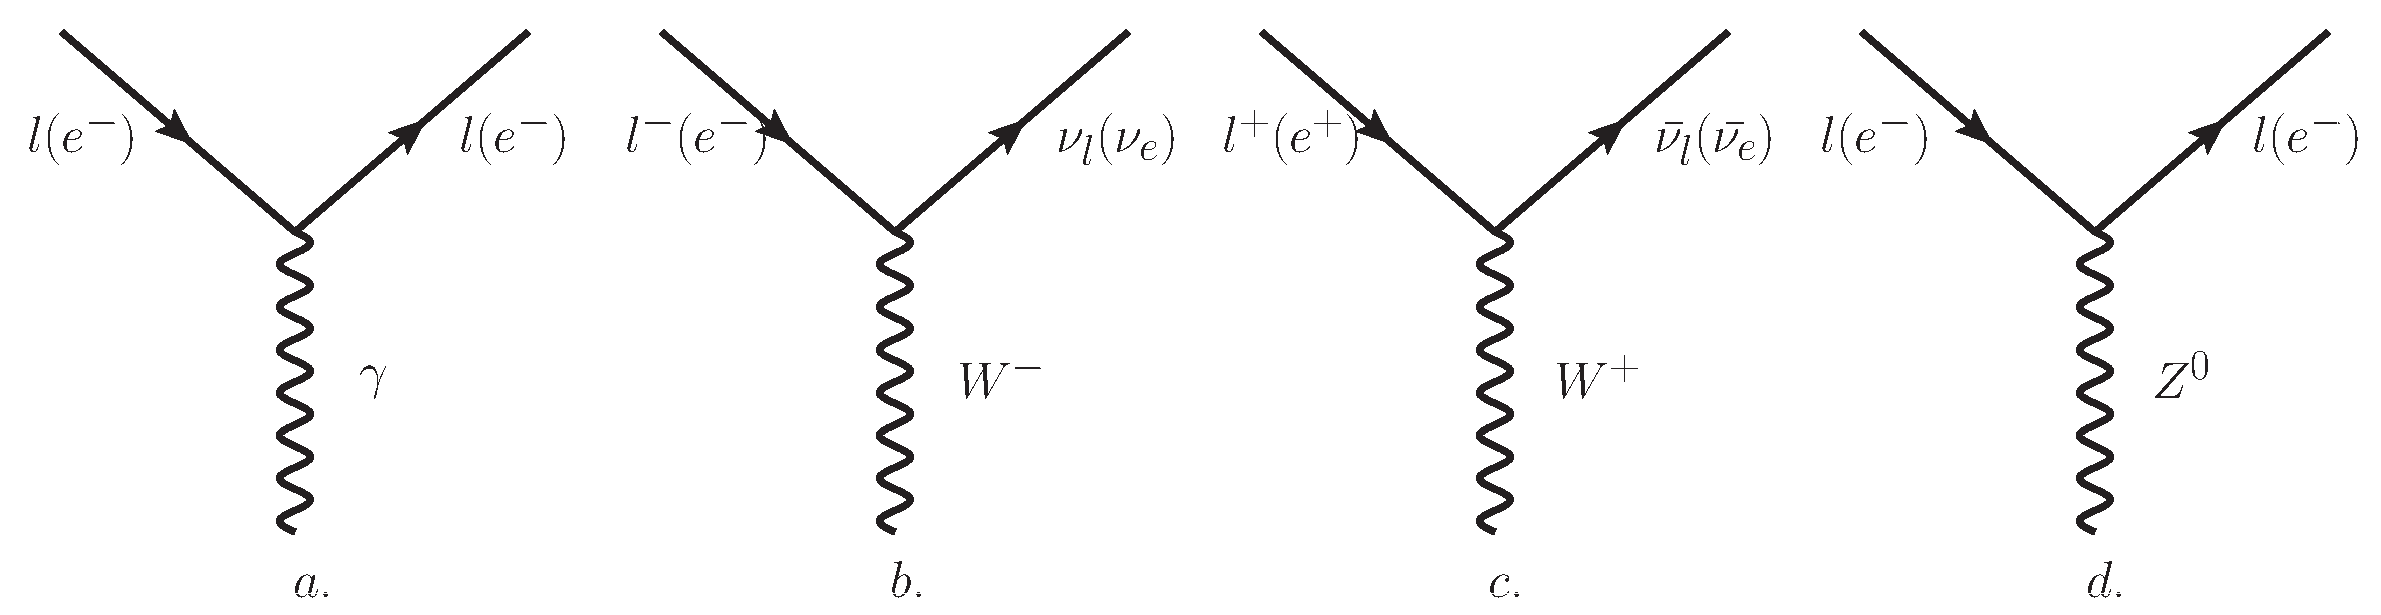
\includegraphics[scale=0.4]{lepton_int}
%%   \caption[Leptons interactions]{Diagrams representing the leptons interactions with the gauge fields; a: EI-electron and photon; b,c,d: WI - first generation leptons.}
%%   \label{lepton_int}
%% \end{figure}

%% The lepton number definition has to be extended when considering the WI. The new definition is given in terms of the generation's weak isospin doublets, thus, electron and electron neutrino have electron number $L_e=1$, muon and muon neutrino have muon number $L_\mu=1$, tau and tau neutrino have tau number $L_\tau=1$. Lepton number conservation, which now is SM wide, implies that leptons have to be created in pairs.

Although all three flavor neutrinos have been observed, their masses remain unknown and only some estimations have been made\cite{nu_mass}. The main reason is that the flavor eigenstates are not the same as the mass eigenstates which implies that when a neutrino is created its mass state is a linear combination of the three mass eigenstates and experiments can only probe the squared difference of the masses. The Pontecorvo-Maki-Nakagawa-Sakata (PMNS) mixing matrix encodes the relationship between flavor and mass eigenstates.
\begin{center}
\begin{table}[h]
\centering
\footnotesize
\begin{tabular}{lcccccc} \hline
Lepton                      & Q(e) & $T_3$&$L_e$ & $L_\mu$ & $L_\tau$ & Lifetime (s)                \\ \hline
Electron (e)                & -1   & -1/2 & 1    & 0       & 0        & Stable                      \\ %\hline
Electron neutrino($\nu_e$)  & 0    &  1/2 & 1    & 0       & 0        & Unknown                     \\ %\hline
Muon ($\mu$)                & -1   & -1/2 & 0    & 1       & 0        & $2.19\times10^{-6}$\\ %\hline
Muon neutrino ($\nu_\mu$)   & 0    &  1/2 & 0    & 1       & 0        & Unknown                     \\ %\hline
Tau ($\tau$)                & -1   & -1/2 & 0    & 0       & 1        & $290.3\times10^{-15}$    \\ %\hline
Tau neutrino ($\tau_\mu$)   & 0    &  1/2 & 0    & 0       & 1        & Unknown                     \\ \hline
\end{tabular}
\caption[Lepton properties.]{Lepton properties\cite{pdg}. Q: electric charge, $T_3$: weak isospin. Only left-handed leptons and right-handed anti-leptons participate in the WI. Anti-particles with inverted $T_3$, Q and lepton number complete the leptons set but are not listed. Right-handed leptons and left-handed anti-leptons, neither listed, form weak isospin singlets with $T_3=0$ and do not take part in the weak interaction.}\label{leptons}
\end{table}
\end{center}

\subsubsection{Quarks}

Quarks are the basic constituents of protons and neutrons. The way quarks join to form bound states, called \ti{hadrons}, is through the SI. Quarks are affected by all the fundamental interactions which means that they carry all the four types of charges: color, electric charge, weak isospin and mass.

\begin{center}
\begin{table}[h!]
\centering
\footnotesize
\begin{tabular}{lcccccccccc} \hline
Flavor     & Q(e) & $I_3$ & $T_3$  & B   & C & S  & T & B'  & Y    & Color \\ \hline
Up (u)     & 2/3  & 1/2   &  1/2   & 1/3 & 0 & 0  & 0 & 0   & 1/3  & r,b,g \\ %\hline
Charm (c)  & 2/3  & 0     &  1/2   & 1/3 & 1 & 0  & 0 & 0   & 4/3  & r,b,g \\ %\hline
Top(t)     & 2/3  & 0     &  1/2   & 1/3 & 0 & 0  & 1 & 0   & 4/3  & r,b,g \\ \hline
Down(d)    & -1/3 & -1/2  & -1/2   & 1/3 & 0 & 0  & 0 & 0   & 1/3  & r,b,g \\ %\hline
Strange(s) & -1/3 & 0     & -1/2   & 1/3 & 0 & -1 & 0 & 0   & -2/3 & r,b,g \\ %\hline
Bottom(b)  & -1/3 & 0     & -1/2   & 1/3 & 0 & 0  & 0 & -1  & -2/3 & r,b,g \\ \hline
\end{tabular}
\caption[Quark properties.]{Quark properties \cite{pdg}. Q: electric charge, $I_3$: isospin, $T_3$: weak isospin, B: baryon number, C: charmness, S: strangeness, T: topness, B': bottomness, Y: hypercharge. Anti-quarks posses the same mass and spin as quarks but all charges (color, flavor numbers) have opposite sign.}\label{quarks}
\end{table}
\end{center}

Table \ref{quarks} summarizes the features of quarks, among which the most remarkable is their fractional electric charge. Note that fractional charge is not a problem, given that quarks are not found isolated, but serves to explain how composed particles are formed out of two or more valence quarks\footnote{Hadrons can contain an indefinite number of virtual quarks and gluons, known as the quark and gluon sea, but only the valence quarks determine hadrons' quantum numbers.}.

Color charge is responsible for the SI between quarks and is the symmetry ($SU(3)_C$) that defines the formalism to describe SI. There are three colors: red (r), blue (b) and green (g) and their corresponding three anti-colors; thus each quark carries one color unit while anti-quarks carries one anti-color unit. As explained in Section \ref{fund_inter}, quarks are not allowed to be isolated due to the color confinement effect, hence, their features have been studied indirectly by observing their bound states created when

\begin{itemize}
\item one quark with a color charge is attracted by an anti-quark with the corresponding anti-color charge forming a colorless particle called a \ti{meson.}
\item three quarks (anti-quarks) with different color (anti-color) charges are attracted among them forming a colorless particle called a \ti{baryon (anti-baryon).}          
\end{itemize}

In practice, when a quark is left alone isolated a process called \ti{hadronization} occurs where the quark emits gluons (see Section \ref{sec:gb}) which eventually will generate new quark-antiquark pairs and so on; those quarks will recombine to form hadrons that will decay into leptons. This proliferation of particles looks like a \ti{jet} coming from the isolated quark. More details about the hadronization process and jet structure will be given in chapter\ref{ch:gensimreco}.         

In the first version of the quark model (1964), M. Gell-Mann\cite{gellman} and G. Zweig\cite{zweig,zweig2} developed a consistent way to classify hadrons according to their properties. Only three quarks (u, d, s) were involved in a scheme in which all baryons have baryon number B=1 and therefore quarks have B=1/3; non-baryons have B=0. Baryon number is conserved in SI and EI which means that single quarks cannot be created but in pairs $q-\bar{q}$.

The scheme organizes baryons in a two-dimensional space ($I_3$ - Y); Y (hypercharge) and $I_3$ (isospin) are quantum numbers related by the Gell-Mann-Nishijima formula\cite{gell_ni,gell_ni2}:
\begin{equation}
Q=I_3 + \frac{Y}{2}
\label{gmn}
\end{equation}

\noindent where $Y=B+S+C+T+B'$ are the quantum numbers listed in Table \ref{quarks}. 

There are six quark flavors organized in three generations (see Table \ref{flav_gen}) following a mass hierarchy which, again, implies that higher generations decay to first generation quarks.

\begin{center}
\begin{table}[h!]
\centering
\footnotesize
\begin{tabular}{ccccccccccc} \hline
                          &     \multicolumn{3}{c}{Quarks}                       & $T_3$              & $Y_W$&  \multicolumn{3}{c}{Leptons}                                              & $T_3$                    & $Y_W$\\\hline
Doublets                  & $\binom{u}{d'}_L$& $\binom{c}{s'}_L$& $\binom{t}{b'}_L$& $\binom{1/2}{-1/2}$& 1/3  & $\binom{\nu_e}{e}_L$ & $\binom{\nu_\mu}{\mu}_L$& $\binom{\nu_\tau}{\tau}_L$& $\binom{1/2}{-1/2}$ & -1    \\ %\hline \\%\hline 
\multirow{2}{*}{Singlets} & $u_R$            & $c_R$            & $t_R$            & 0                  & 4/3 & $\nu_{eR}$           & $\nu_{\mu R}$           & $\nu_{\tau R}$            &                     &       \\ % \\
                          & $d'_R$           & $s'_R$           & $b'_R$           & 0                  & -2/3 & $e_R$                & $\mu_R$                 & $\tau_R$                  & 0                   & -2   \\ \hline % \\ \hline
%% Leptons                   &                      &                         &                           &                     &       \\ \hline
%% Doublets                  & $\binom{\nu_e}{e}_L$ & $\binom{\nu_\mu}{\mu}_L$& $\binom{\nu_\tau}{\tau}_L$& $\binom{1/2}{-1/2}$ & -1    \\%\hline 
%% \multirow{2}{*}{Singlets} & $\nu_{eR}$           & $\nu_{\mu R}$           & $\nu_{\tau R}$            &                     &       \\
%%                           & $e_R$                & $\mu_R$                 & $\tau_R$                  & 0                   & -2   \\ \hline
\end{tabular}
\caption[Fermion weak isospin and weak hypercharge multiplets.]{Fermion weak isospin and weak hypercharge multiplets. Weak hypercharge is calculated through the Gell-Mann-Nishijima formula \ref{gmn} but using the weak isospin and charge for quarks.}\label{T3Y}
\end{table}
\end{center}

Isospin doublets of quarks are also defined (see Table \ref{T3Y}), and same as for neutrinos, the WI eigenstates are not the same as the mass eigenstates which means that members of different quark generations are connected by the WI mediator; thus, up-type quarks are coupled not to down-type quarks (the mass eigenstates) directly but to a superposition of down-type quarks $(q'_d; the weak eigenstates)$ via WI according to: 

$$q'_d = V_{CKM}\hspace{0.1cm}q_d$$
\begin{equation}
\begin{pmatrix}d'\\ s'\\ b'\end{pmatrix}=\begin{pmatrix} V_{ud} & V_{us} & V_{ub}\\ V_{cd} & V_{cs} & V_{cb}\\ V_{td} & V_{ts} & V_{tb}\end{pmatrix}\begin{pmatrix}d\\s\\b\end{pmatrix}
\label{eq:qmixing}
\end{equation}

\noindent where $V_{CKM}$ is known as Cabibbo-Kobayashi-Maskawa (CKM) mixing matrix\cite{C,KM} given by  

\begin{equation}
\begin{pmatrix}
|V_{ud}| & |V_{us}| & |V_{ub}| \\
|V_{cd}| & |V_{cs}| & |V_{cb}| \\
|V_{td}| & |V_{ts}| & |V_{tb}|
\end{pmatrix} = \begin{pmatrix}
0.97427 \pm 0.00015 & 0.22534 \pm 0.00065 & 0.00351^{+0.00015}_{-0.00014} \\
0.22520 \pm 0.00065 & 0.97344 \pm 0.00016 & 0.0412^{+0.0011}_{-0.0005} \\
0.00867^{+0.00029}_{-0.00031} & 0.0404^{+0.0011}_{-0.0005} & 0.999146^{+0.000021}_{-0.000046}
\end{pmatrix}.
\label{eq:ckm}
\end{equation}

\begin{figure}[!h]
  \centering
  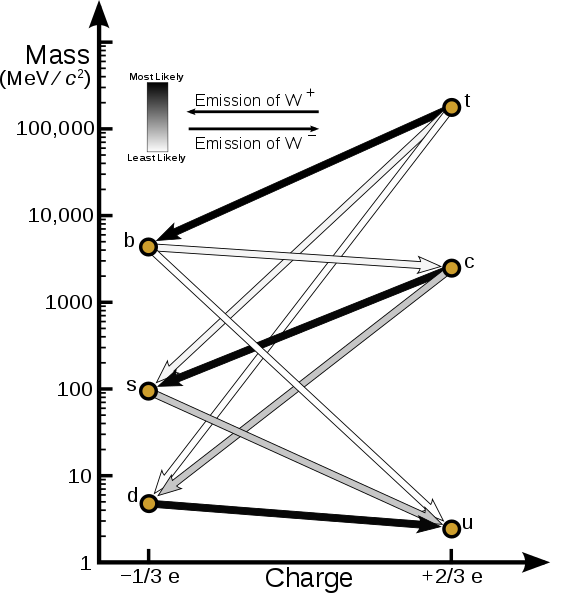
\includegraphics[scale=0.3]{quarks_decay}
  %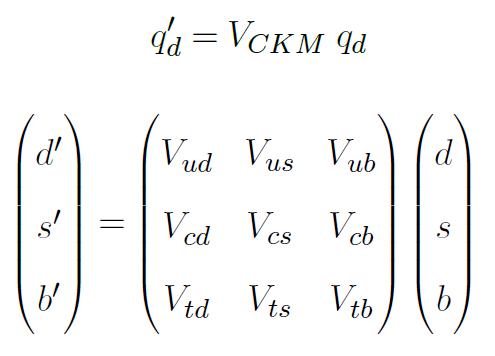
\includegraphics[width=0.45\textwidth]{ckm}
  \caption[Transformations between quarks]{Transformations between quarks through the exchange of a WI. Higher generations quarks decay to first generation quarks by emitting a W boson. The arrow color indicates the likelihood of the transition according to the grey scale in the top left side which represent the CKM matrix parameters\cite{ckm}.}
  \label{quarks_decay}
\end{figure}

The weak decays of quarks are represented in the diagram of Figure \ref{quarks_decay}; again the CKM matrix plays a central role since it contains the probabilities for the different quark decay channels, in particular, note that quark decays are greatly favored between generation members.\\

CKM matrix is a $3\times3$ unitary matrix parametrized by three mixing angles and the \textit{CP-mixing phase}; the latter is the parameter responsible for the Charge-Parity symmetry violation (CP-violation) in the SM. The fact that the top quark decays almost all the time to a bottom quark is exploited in this thesis when making the selection of the signal events by requiring the presence of a jet tagged as a jet coming from a $b$ quark in the final state.% The effect of the \textit{CP-mixing phase} on the cross section of associated production of Higss boson and a single top process is also explored in this thesis.    

\subsection{Fundamental interactions}\label{fund_inter}

\begin{figure}[h!]
  \centering
  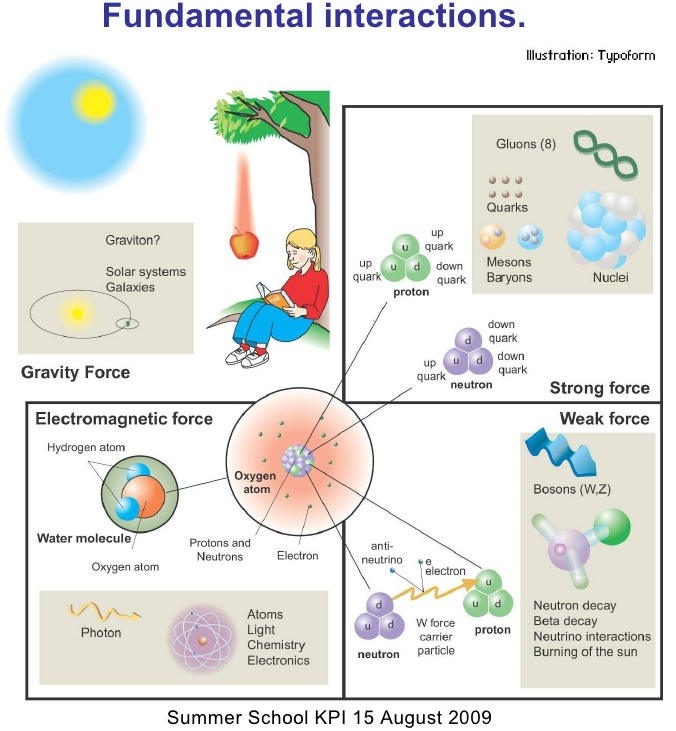
\includegraphics[scale=0.5]{fund_interac}
  \caption[Fundamental interactions in nature.]{Fundamental interactions in nature. Despite the many manifestations of forces in nature, we can track all of them back to one of the fundamental interactions. The most common forces are gravity and electromagnetic given that all of us are subject and experience them in everyday life.}
  \label{fund_interac}
\end{figure}

Even though there are many manifestations of force in nature, like the ones represented in Figure \ref{fund_interac}, we can classify all of them in four fundamental interactions:
\begin{itemize}

\item \textit{Electromagnetic interaction (EI)} affects particles that are \ti{electrically charged,} like electrons and protons.
%It is described by QED, combining quantum mechanics, special relativity and electromagnetism in order to explain how particles with electric charge interact through the exchange of photons, therefore, one says that \ti{Electomagnetic Force} is mediated by \ti{photons}.
Figure \ref{fi_scatt}a. shows a graphical representation, known as \ti{Feynman diagram}, of electron-electron scattering.    

\item \textit{Strong interaction (SI)} described by Quantum Chromodynamics (QCD). Hadrons like the proton and the neutron have internal structure given that they are composed of two or more valence quarks\footnote{Particles made of four and five quarks are exotic states not so common.}. Quarks have fractional electric charge which means that they are subject to electromagnetic interaction and in the case of the proton they should break apart due to electrostatic repulsion; however, quarks are held together inside the hadrons against their electrostatic repulsion by the \ti{Strong Force} through the exchange of \ti{gluons.} The analog to the electric charge is the \ti{color charge}. Electrons and photons are elementary particles as quarks but they don't carry color charge, therefore they are not subject to SI. A Feynman diagram for gluon exchange between quarks is shown in Figure \ref{fi_scatt}b.  

\begin{figure}[h!]
\centering
    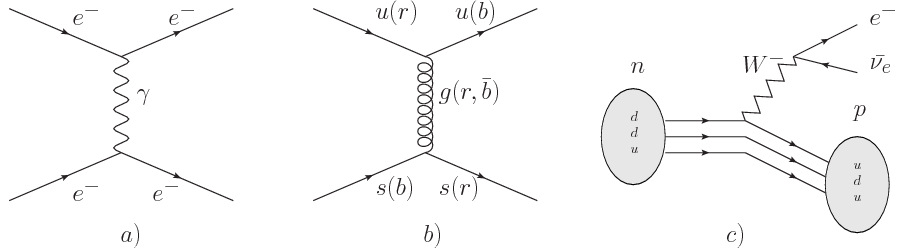
\includegraphics[scale=0.4]{fi_scatt}
\caption[SM interactions diagrams]{Feynman diagrams representing the interactions in SM; a) EI: e-e scattering; b) SI: gluon exchange between quarks ; c) WI: $\beta$-decay }
\label{fi_scatt}
\end{figure}

\item \textit{Weak interaction (WI)} described by the weak theory (WT), is responsible, for instance, for the radioactive decay in atoms and the deuterium production within the sun. Quarks and leptons are the particles affected by the weak interaction; they possess a property called \ti{flavor charge} (see \ref{fermions}) which can be changed by emitting or absorbing one weak force mediator. There are three mediators of the \ti{weak force} known as \ti{Z} boson in the case of electrically neutral flavor changes and \ti{$W^\pm$} bosons in the case of electrically charged flavor changes. The \ti{weak isospin} is the WI analog to electric charge in EI, and color charge in SI, and defines how quarks and leptons are affected by the weak force. Figure \ref{fi_scatt}c. shows the Feynman diagram of $\beta$-decay where a neutron (n) is transformed in a proton (p) by emitting a $W^-$ particle. %Since this thesis is in the frame of the electroweak interaction, a more detailed description of it will be given in Section \ref{sec:EWI}

\item \textit{Gravitational interaction (GI)} described by General Theory of Relativity (GR). It is responsible for the structure of galaxies and black holes as well as the expansion of the universe. As a classical theory, in the sense that it can be formulated without even appeal to the concept of quantization, it implies that the space-time is a continuum and predictions can be made without limitation to the precision of the measurement tools. The latter represents a direct contradiction of the quantum mechanics principles. Gravity is deterministic while quantum mechanics is probabilistic; despite that, efforts to develop a quantum theory of gravity have predicted the \ti{graviton} as mediator of the gravitational force\footnote{Actually a wide variety of theories have been developed in an attempt to describe gravity; some famous examples are string theory and supergravity.}.     
\end{itemize}

\begin{center}
\begin{table}[h!]
\centering
\scriptsize
\begin{tabular}{llm{1.2cm}ll}\hline%\hline
Interaction            & Acts on                         & Relative strength & Range (m)  & Mediators \\ \hline
Electromagnetic (QED)  & Electrically charged particles  & $10^{-2}$         & Infinite   & Photon    \\%\hline
Strong          (QCD)  & Quarks and gluons               & 1                 & $10^{-15}$ & Gluon     \\%\hline
Weak            (WI)   & Leptons and quarks              & $10^{-6}$         & $10^{-18}$ & \wpm, Z   \\%\hline
Gravitational   (GI)   & Massive particles               & $10^{-39}$        & Infinite   & Graviton  \\\hline
\end{tabular}
\caption[Fundamental interactions features.]{Fundamental interactions features\cite{hyperphys}. }\label{fund_inter_feat}
\end{table}
\end{center}

Table \ref{fund_inter_feat} summarizes the main features of the fundamental interactions. The relative strength of the fundamental forces reveals the meaning of strong and weak; in a context where the relative strength of the SI is 1, the EI is about hundred times weaker and WI is about million times weaker than the SI. A good description on how the relative strength and range of the fundamental interactions are calculated can be found in References \cite{hyperphys,matt}. In the everyday life, only EI and GI are explicitly experienced due to the range of these interactions; \ie, at the human scale distances only EI and GI have appreciable effects, in contrast to SI which at distances greater than $10^{-15}$m become negligible.\\                     

\subsection{Gauge invariance.}
QED was built successfully on the basis of the classical electrodynamics theory (CED) of Maxwell and Lorentz, following theoretical and experimental requirements imposed by

\begin{itemize}
\item Lorentz invariance: independence on the reference frame.  
\item Locality: interacting fields are evaluated at the same space-time point to avoid action at a distance. 
\item Renormalizability: physical predictions are finite and well defined. 
\item Particle spectrum, symmetries and conservation laws already known must emerge from the theory.
\item Local gauge invariance.
\end{itemize}

The gauge invariance requirement reflects the fact that the fundamental fields cannot be directly measured but associated fields which are the observables. Electric (\textbf{E}) and magnetic (\textbf{B}) fields in CED are associated with the electric scalar potential \ti{V} and the vector potential \textbf{A}. In particular, \textbf{E} can be obtained by measuring the change in the space of the scalar potential (\textbf{$\Delta$}V); however, two scalar potentials differing by a constant \ti{f} correspond to the same electric field. The same happens in the case of the vector potential \textbf{A}; thus, different configurations of the associated fields result in the same set of values of the observables. The freedom in choosing one particular configuration is known as \ti{gauge freedom}; the transformation law connecting two configurations is known as \ti{gauge transformation} and the fact that the observables are not affected by a gauge transformation is called \ti{gauge invariance}.

When the gauge transformation:  

\begin{align}\label{cov_der}
\textbf{A} \to &\textbf{A} -\Delta f\nonumber\\
V \to & V - \frac{\partial f}{\partial t}
\end{align}

\noindent is applied to Maxwell equations, they are still satisfied and the fields remain invariant. Thus, CED is invariant under gauge transformations and is called a \ti{gauge theory}. The set of all gauge transformations form the \ti{symmetry group} of the theory, which according to the group theory, has a set of \ti{group generators}. The number of group generators determine the number of \ti{gauge fields} of the theory.

As mentioned in the first lines of Section \ref{secc:SM}, QED has one symmetry group (U(1)) with one group generator (the Q operator) and one gauge field (the electromagnetic field $A^\mu$). In CED there is not a clear definition, beyond the historical convention, of which fields are the fundamental and which are the associated, but in QED the fundamental field is $A^\mu$. When a gauge theory is quantized, the gauge fields are quantized and their quanta are called \ti{gauge bosons}. The word boson characterizes particles with integer spin which obey Bose-Einstein statistics.     

As will be detailed in Section \ref{sec:EWI}, interactions between particles in a system can be obtained by considering first the Lagrangian density of free particles in the system, which of course is incomplete because the interaction terms have been left out, and demanding global phase transformation invariance. Global phase transformation invariance means that a gauge transformation is performed identically to every point in the space\footnote{Here space corresponds to the 4-dimensional space \ie space-time.} and the Lagrangian remains invariant. Then, the global transformation is promoted to a local phase transformation (this time the gauge transformation depends on the position in space) and again invariance is required.

Due to the space dependence of the local transformation, the Lagrangian density is not invariant anymore. In order to reinstate the gauge invariance, the gauge covariant derivative is introduced in the Lagrangian and with it the gauge field responsible for the interaction between particles in the system. The new Lagrangian density is gauge invariant, includes the interaction terms needed to account for the interactions and provides a way to explain the interaction between particles through the exchange of the gauge boson.

This recipe was used to build QED and the theories that aim to explain the fundamental interactions.   

\subsection{Gauge bosons}\label{sec:gb}

The importance of the gauge bosons comes from the fact that they are the force mediators or force carriers. The features of the gauge bosons reflect those of the fields they represent and they are extracted from the Lagrangian density used to describe the interactions. In Section \ref{sec:EWI}, it will be shown how the gauge bosons of the EI and WI emerge from the electroweak Lagrangian. The SI gauge bosons features are also extracted from the SI Lagrangian but it is not detailed in this document. The main features of the SM gauge bosons will be briefly presented below and summarized in Table \ref{gauge_boson}.

\begin{itemize} 
\item \textbf{Photon}.
EI occurs when the photon couples to (is exchanged between) particles carrying electric charge; however,
The photon itself does not carry electric charge, therefore, there is no coupling between photons. Given that the photon is massless the EI is of infinite range, \ie, electrically charged particles interact even if they are located far away one from each other; this also implies that photons always move with the speed of light. 

\item \textbf{Gluon}. SI is mediated by gluons which just as photons are massless. They carry one unit of color charge and one unit of anticolor charge, hence, gluons can couple to other gluons. As a result, the range of the SI is not infinite but very short due to the attraction between gluons, giving rise to the \ti{color confinement} which explains why color charged particles cannot be isolated but live within composite particles, like quarks inside protons. 

\item  \textbf{W, Z}. %The WI mediators,
$\wpm$ and Z, are massive which explains their short-range. Given that the WI is the only interaction that can change the flavor of the interacting particles, the W boson is the responsible for the nuclear transmutation where a neutron is converted into a proton or vice versa with the involvement of an electron and a neutrino (see Figure \ref{fi_scatt}c). The Z boson is the responsible for the neutral weak processes like neutrino elastic scattering where no electric charge but momentum transference is involved. WI gauge bosons carry isospin charge which makes interaction between them possible.  
\end{itemize}

\begin{center}
\begin{table}[h!]
\centering
\scriptsize
\begin{tabular}{llllll}\hline%\hline
Interaction            & Mediator          & Electric charge (e) & Color charge & Weak Isospin & mass (GeV/c$^2$)   \\ \hline
Electromagnetic        & Photon ($\gamma$) & 0                   & No           & 0            & 0                  \\%\hline
Strong                 & Gluon (g)         & 0                   & Yes -octet   & No           & 0                  \\%\hline
\multirow{2}{*}{Weak}  & \wpm              & $\pm 1$             & No           & $\pm 1$      & 80.385 $\pm$ 0.015 \\%\hline
                       & Z                 & 0                   & No           & 0            & 91.188 $\pm$ 0.002 \\\hline
\end{tabular}
\caption[SM gauge bosons.]{SM gauge bosons main features\cite{pdg}.}\label{gauge_boson}
\end{table}
\end{center}

\section{Electroweak unification and the Higgs mechanism}\label{sec:EWI}

Physicists dream of building a theory that contains all the interactions in one single interaction, \ie, showing that at some scale in energy all the four fundamental interactions are unified and only one interaction emerges in a \ti{Theory of everything}. The first sign of the feasibility of such unification came from success in the construction of the CED. Einstein spent years trying to reach that full unification, which by 1920 only involved electromagnetism and gravity, with no success; however, a new partial unification was achieved in the 1960's, when S.Glashow\cite{glashow}, A.Salam\cite{salam} and S.Weinberg \cite{weinberg} independently proposed that electromagnetic and weak interactions are two manifestations of a more general interaction called \ti{electroweak interaction (EWI)}. EWI was developed by following the useful prescription provided by QED and the gauge invariance principles.

\begin{figure}[h!]
  \centering
  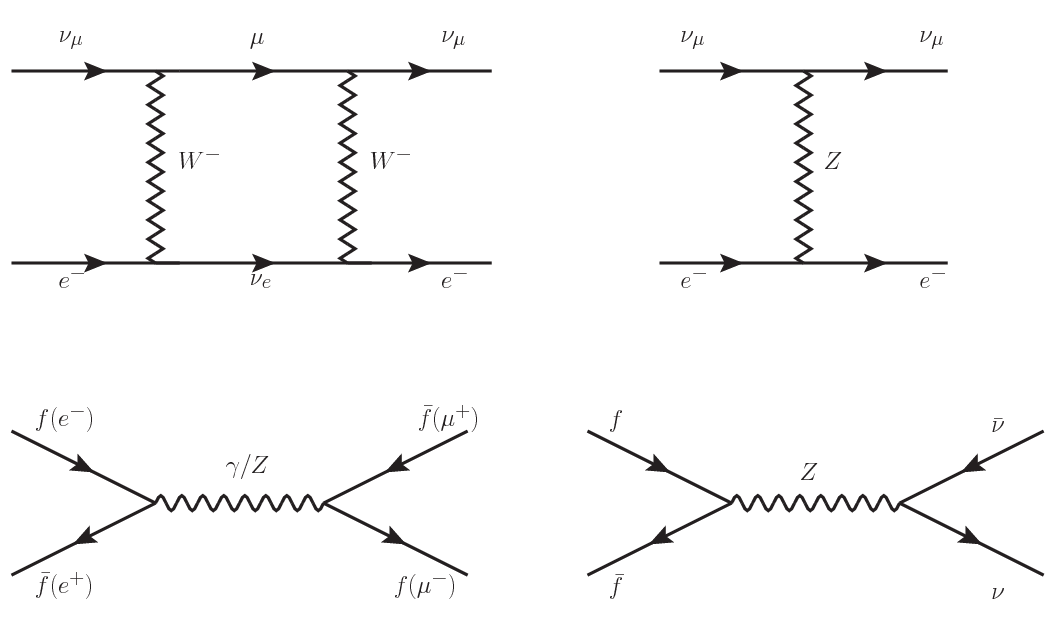
\includegraphics[scale=0.4]{nc}
  \caption[Neutral current processes]{Top: $\nu_{\mu}-e^-$ scattering going through charged currents (left) and neutral currents (right). Bottom: neutral current processes for charged fermions (left) and involving neutrinos (right). While neutral current processes involving only charged fermions can proceed through EI or WI, those involving neutrinos can only proceed via WI.}% The former can be seen as an indication that at some level WI and EI are closely connected.}
         \label{nc}
\end{figure}

The \ti{classic} weak theory developed by Fermi, did not have the concept of the W boson but instead it was treated as a point interaction with the dimensionful constant $G_F$ associated with it. It works really well at low energies very far off the W mass shell. When going up in energy, the theory of weak interactions involving the W boson is capable of explaining the $\beta$-decay and in general the processes mediated by \wpm bosons. However, there were some processes like the \ti{$\nu_\mu - e$ scattering} which would require the exchange of two W bosons (see Figure \ref{nc} top diagrams) giving rise to divergent loop integrals and then non-finite predictions. The EWI theory, by including neutral currents involving fermions via the exchange of a neutral bosons Z, overcomes those divergences and the predictions become realistic.

Neutral weak interaction vertices conserve flavor in the same way as the electromagnetic vertices do, but additionally, the Z boson can couple to neutrinos which implies that processes involving charged fermions can proceed through EI or WI but processes involving neutrinos can proceed only through WI.   

The prescription to build a gauge theory of the WI consists of proposing a free field Lagrangian density that includes the particles involved; next, by requesting invariance under global phase transformations first and generalizing to local phase transformations invariance later, the conserved currents are identified and interactions are generated by introducing gauge fields. Given that the goal is to include the EI and WI in a single theory, the group symmetry considered should be a combination of $SU(2)_L$ and $U(1)_{em}$ , however the latter cannot be used directly because the EI treats left and right-handed particles indistinctly in contrast to the former. Fortunately, the weak hypercharge, which is a combination of the weak isospin and the electric charge (Eqn. \ref{gmn}) is suitable to be used since it is conserved by the  EI and WI. Thus, the symmetry group to be considered is

\begin{equation}
G\equiv SU(2)_L\otimes U(1)_Y
\end{equation}

 The following treatment applies to any of the fermion generations, but for simplicity the first generation of leptons will be considered\cite{peskin,mandl,halzen,pich}.\\

Given the first generation of leptons 

\begin{equation}\label{first_gen}
\psi_1 = \binom{\nu_e}{e^-}_L , \qquad \psi_2= \nu_{eR}, \qquad \psi_3= e^-_R
\end{equation}

\noindent the charged fermionic currents are given by

\beqn\label{fermion_currents}
J_\mu \equiv  J_\mu^+ = \bar{\nu}_{eL} \gamma_\mu e_L, \qquad J_\mu^\dagger \equiv J_\mu^- = \bar{e}_L \gamma_\mu \nu_{eL} 
\eeqn

\noindent and the free Lagrangian is given by

\begin{equation}\label{lo}
\Lagr_0 = \sum_{j=1}^3 i\overline{\psi}_j(x)\gamma^\mu \partial_\mu \psi_j(x).
\end{equation}

Mass terms are included directly in the QED free Lagrangians since they preserve the invariance under the symmetry transformations involved which treat left and right handed particles similarly, however mass terms of the form

\beqn 
m_W^2W_\mu^\dagger(x)W^\mu(x) + \frac{1}{2}m_Z^2Z_\mu(x)Z^\mu(x) -m_e\bar{\psi_e}(x)\psi_e(x)
\eeqn
\noindent which represent the mass of \wpm, Z and electrons, are not invariant under G transformations, therefore the gauge fields described by the EWI are in principle massless.

Experiments have shown that the EWI gauge fields are not massless\cite{wmass1,wmass2,zmass1,zmass2}; however, they have to acquire mass through a mechanism compatible with the gauge invariance; that mechanism is known as the \ti{Higgs mechanism} and will be considered later in this Section. The global transformations in the combined symmetry group G can be written as

\begin{align}\label{G_transf}
\psi_1(x) \xrightarrow[]{G}\psi'_1(x)\equiv &U_YU_L\psi_1(x),\nonumber\\ 
\psi_2(x) \xrightarrow[]{G}\psi'_2(x)\equiv &U_Y\psi_2(x),\\
\psi_3(x) \xrightarrow[]{G}\psi'_3(x)\equiv &U_Y\psi_3(x)\nonumber
\end{align}
\noindent where $U_L$ represent the $SU(2)_L$ transformation acting only on the weak isospin doublet and $U_Y$ represent the $U(1)_Y$ transformation acting on all the weak isospin multiplets. Explicitly
\beqn
U_L\equiv \exp \left(i\frac{\sigma_i}{2}\alpha^i\right), \qquad U_Y\equiv \exp(iy_i\beta) \qquad (i=1,2,3)
\eeqn
\noindent with $\sigma_i$ the Pauli matrices and $y_i$ the weak hypercharges. In order to promote the transformations from global to local while keeping the invariance, it is required that $\alpha^i=\alpha^i(x)$, $\beta=\beta(x)$ and the replacement of the ordinary derivatives by the covariant derivatives

\begin{align}\label{cov_der2}
D_\mu \psi_1(x) \equiv &\left[\partial_\mu + ig\sigma_i W_\mu^i(x)/2+ ig'y_1B_\mu(x)\right]\psi_1(x)\nonumber\\ 
D_\mu \psi_2(x) \equiv &\left[\partial_\mu + ig'y_2B_\mu(x)\right]\psi_2(x)\\
D_\mu \psi_3(x) \equiv &\left[\partial_\mu + ig'y_3B_\mu(x)\right]\psi_3(x)\nonumber 
\end{align}

\noindent introducing in this way four gauge fields, $W_\mu^i(x)$ and $B_\mu(x)$, in the process. The covariant derivatives (Eqn. \ref{cov_der2}) are required to transform in the same way as fermion fields $\psi_i(x)$ themselves, therefore, the gauge fields transform as:

\begin{align}\label{f_transf}
B_\mu(x) \xrightarrow[]{G} B_\mu'(x)\equiv & B_\mu(x)
- \frac{1}{g'}\partial_\mu\beta(x) \nonumber\\
W^i_\mu(x) \xrightarrow[]{G} W_\mu^{i\prime}(x)\equiv & W^i_\mu(x) - \frac{i}{g}\partial_\mu \alpha_i(x) - \varepsilon_{ijk}\alpha_i(x)W^i_\mu(x).
\end{align}

The G invariant version of the Lagrangian density \ref{lo} can be written as

\begin{equation}\label{linv}
\Lagr_0 = \sum_{j=1}^3 i\overline{\psi}_j(x)\gamma^\mu D_\mu \psi_j(x)
\end{equation}

\noindent where free massless fermion and gauge fields and fermion-gauge boson interactions are included. The EWI Lagrangian density must additionally include kinetic terms for the gauge fields ($\Lagr_G$) which are built from the field strengths, according to

\begin{align}
B_{\mu\nu}(x)   \equiv & \partial_\mu B_\nu -  \partial_\nu B_\mu \label{B_tensor} \\ 
W^i_{\mu\nu}(x) \equiv & \partial_\mu W^i_\nu(x) - \partial_\nu W^i_\mu(x) - g\varepsilon^{ijk}W^j_\mu W^k_\nu \label{W_tensor}
\end{align}

\noindent the last term in Eqn. \ref{W_tensor} is added in order to hold the gauge invariance; therefore,

\beqn\label{lg}
\Lagr_G = -\frac{1}{4}B_{\mu\nu}(x)B^{\mu\nu}(x)-\frac{1}{4}W^i_{\mu\nu}(x)W_i^{\mu\nu}(x)
\eeqn

\noindent which contains not only the free gauge fields contributions, but also the gauge fields self-interactions and interactions among them.

The three weak isospin conserved currents resulting from the $SU(2)_L$ symmetry are given by

\beqn
J_\mu^i(x)=\frac{1}{2}\bar{\psi_1}(x)\gamma_\mu \sigma^i \psi_1(x) 
\eeqn

\noindent while the weak hypercharge conserved current resulting from the $U(1)_Y$ symmetry is given by 

\beqn
J_\mu^Y = \sum_{j=1}^3 \overline{\psi}_j(x)\gamma_\mu y_j\psi_j(x)
\eeqn

In order to evaluate the electroweak interactions modeled by an isotriplet field $W^i_\mu$ that couples to isospin currents $J^i_\mu$ with strength $g$ and additionally the singlet field $B_\mu$ which couples to the weak hypercharge current $J_\mu^Y$ with strength $g'/2$. The interaction Lagrangian density to be considered is

\beqn
\Lagr_I = -gJ^{i\mu}(x)W_\mu^i(x)- \frac{g'}{2}J^{Y\mu}(x)B_\mu(x)
\eeqn

%\noindent written in terms of the physical fields $\wpm_\mu$, $Z_\mu$ and $A_\mu$.

Note that the weak isospin currents are not the same as the charged fermionic currents that were used to describe the WI (Eqn. \ref{fermion_currents}), since the weak isospin eigenstates are not the same as the mass eigenstates, but they are closely related

\beqn\label{fermion_currents2}
J_\mu = \frac{1}{2}(J_\mu^1 + iJ_\mu^2) ,  \qquad  J_\mu^\dagger = \frac{1}{2}(J_\mu^1 - iJ_\mu^2).
\eeqn

The same happens with the gauge fields $W^i_\mu$ which are related to the mass eigenstates \wpm by     

\beqn\label{wboson_mass_eigen}
W^+_\mu = \frac{1}{\sqrt{2}}(W_\mu^1-iW_\mu^2), \qquad W^-_\mu = \frac{1}{\sqrt{2}}(W_\mu^1+iW_\mu^2).
\eeqn

The fact that there are three weak isospin conserved currents is an indication that in addition to the charged fermionic currents, which couple charged to neutral leptons, there should be a neutral fermionic current that does not involve electric charge exchange; therefore, it couples neutral fermions or fermions of the same electric charge. The third weak isospin current contains a term that is similar to the electromagnetic current ($j_\mu^{em}$), indicating that there is a relation between them  and resembling the Gell-Mann-Nishijima formula \ref{gmn} adapted to electroweak interactions
\begin{equation}
Q=T_3 + \frac{Y_W}{2}.
\label{gmn_ew}
\end{equation}

Just as Q generates the $U(1)_{em}$ symmetry, the weak hypercharge generates the $U(1)_Y$ symmetry as said before. It is possible to write the relationship in terms of the currents as

\beqn \label{neutral_currents}
j_\mu^{em} = J_\mu^3  + \frac{1}{2}J_\mu^Y.
\eeqn

The neutral gauge fields $W^3_\mu$ and $B_\mu$ cannot be directly identified with the $Z$ and the photon fields since the photon interacts similarly with left and right-handed fermions; however, they are related through a linear combination given by

\begin{align}\label{neutral_fields}
A_\mu = &  B_\mu \cos\theta_W + W^3_\mu \sin\theta_W \\ 
Z_\mu = & -B_\mu \sin\theta_W + W^3_\mu \cos\theta_W \nonumber 
\end{align}

\noindent where $\theta_W$ is known as the \ti{Weinberg angle.} The interaction Lagrangian is now given by
\begin{align}
\Lagr_I =-\frac{g}{\sqrt{2}}(J^\mu W_\mu^+ + J^{\mu\dagger}W_\mu^-) -\left(g\sin\theta_W J_\mu^3 + g'\cos\theta_W \frac{J_\mu^Y}{2} \right)A^\mu \\ \nonumber
- \left(g\cos\theta_W J_\mu^3 - g'\sin\theta_W \frac{J_\mu^Y}{2} \right)Z^\mu 
\end{align}

\noindent the first term is the weak charged current interaction, while the second term is the electromagnetic interaction under the condition
\beqn
g\sin\theta_W = g'\cos\theta_W = e, \quad \frac{g'}{g}= \tan\theta_W  
\eeqn
\noindent contained in the Eqn.\ref{neutral_currents}; the third term is the neutral weak current.\\

Note that the neutral fields transformation given by the Eqn. \ref{neutral_fields} can be written in terms of the coupling constants $g$ and $g'$ as:
\beqn\label{neutral_bosons}
A_\mu= \frac{g'W_\mu^3 + gB_\mu}{\sqrt{g^2+g'^2}}, \qquad  Z_\mu= \frac{gW_\mu^3 - g'B_\mu}{\sqrt{g^2+g'^2}}.
\eeqn

So far, the Lagrangian density describing the non-massive EWI is:
\beqn\label{nmewi_lagr}
\Lagr_{nmEWI}=\Lagr_0 +\Lagr_G
\eeqn
\noindent where fermion and gauge fields have been considered massless because their regular mass terms are manifestly non invariant under G transformations; therefore, masses have to be generated in a gauge invariant way. The mechanism by which this goal is achieved is known as the \ti{Higgs mechanism} and is closely connected to the concept of \ti{spontaneous symmetry breaking.}

\subsection{Spontaneous symmetry breaking (SSB)}

Figure \ref{ssb} left shows a steel nail (top) which is subject to an external force; the form of the potential energy is also shown (bottom).

\begin{figure}[!h]
\centering
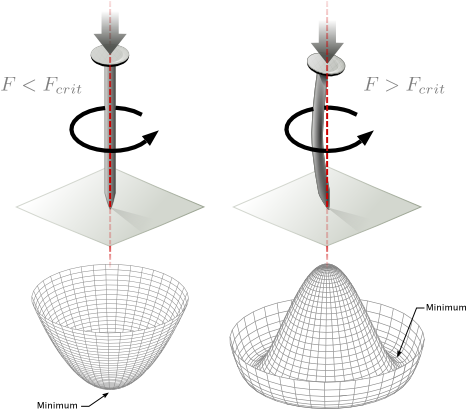
\includegraphics[scale=0.4]{broken_symmetry}
\caption[Spontaneous symmetry breaking mechanism]{Spontaneous symmetry breaking mechanism. The steel nail, subject to an external force (top left), has rotational symmetry with respect to its axis. When the external force overcomes a critical value the nail buckles (top right) choosing a minimal energy state (ground state) and thus \textit{breaking spontaneously the rotational symmetry}. The potential energy (bottom) changes but holds the rotational symmetry; however, an infinite number of asymmetric ground states are generated and circularly distributed in the bottom of the potential\cite{broken_symmetry}.}
\label{ssb}
\end{figure}

Before reaching the critical force value, the system has rotational symmetry with respect to the nail axis; however, after the critical force value is reached the nail buckles (top right). The form of the potential energy (bottom right) changes appearing a set of infinity minima  but preserving its rotational symmetry. Right before the nail buckles there is no indication of the direction the nail will bend because any of the directions are equivalent, but once the nail bends, choosing a direction, an arbitrary minimal energy state (ground state) is selected and it does not share the system's rotational symmetry. This mechanism for reaching an asymmetric ground state is known as \textit{spontaneous symmetry breaking}.       

The lesson from this analysis is that the way to introduce the SSB mechanism into a system is by adding the appropriate potential to it.

Figure \ref{hp2d} shows a plot of the potential $V(\phi)$ in the case of a scalar field $\phi$

\beqn\label{Higgs_potential}
V(\phi)=\mu^2\phi^\dagger\phi + \lambda(\phi^\dagger\phi)^2
\eeqn

If $\mu^2>0$ the potential has only one minimum at $\phi=0$ and describes a scalar field with mass $\mu$. If $\mu^2<0$ the potential has a local maximum at $\phi=0$ and two minima at $\phi=\pm \sqrt{-\mu^2/\lambda}$ which enables the SSB mechanism to work.

\begin{figure}[!h]
\centering
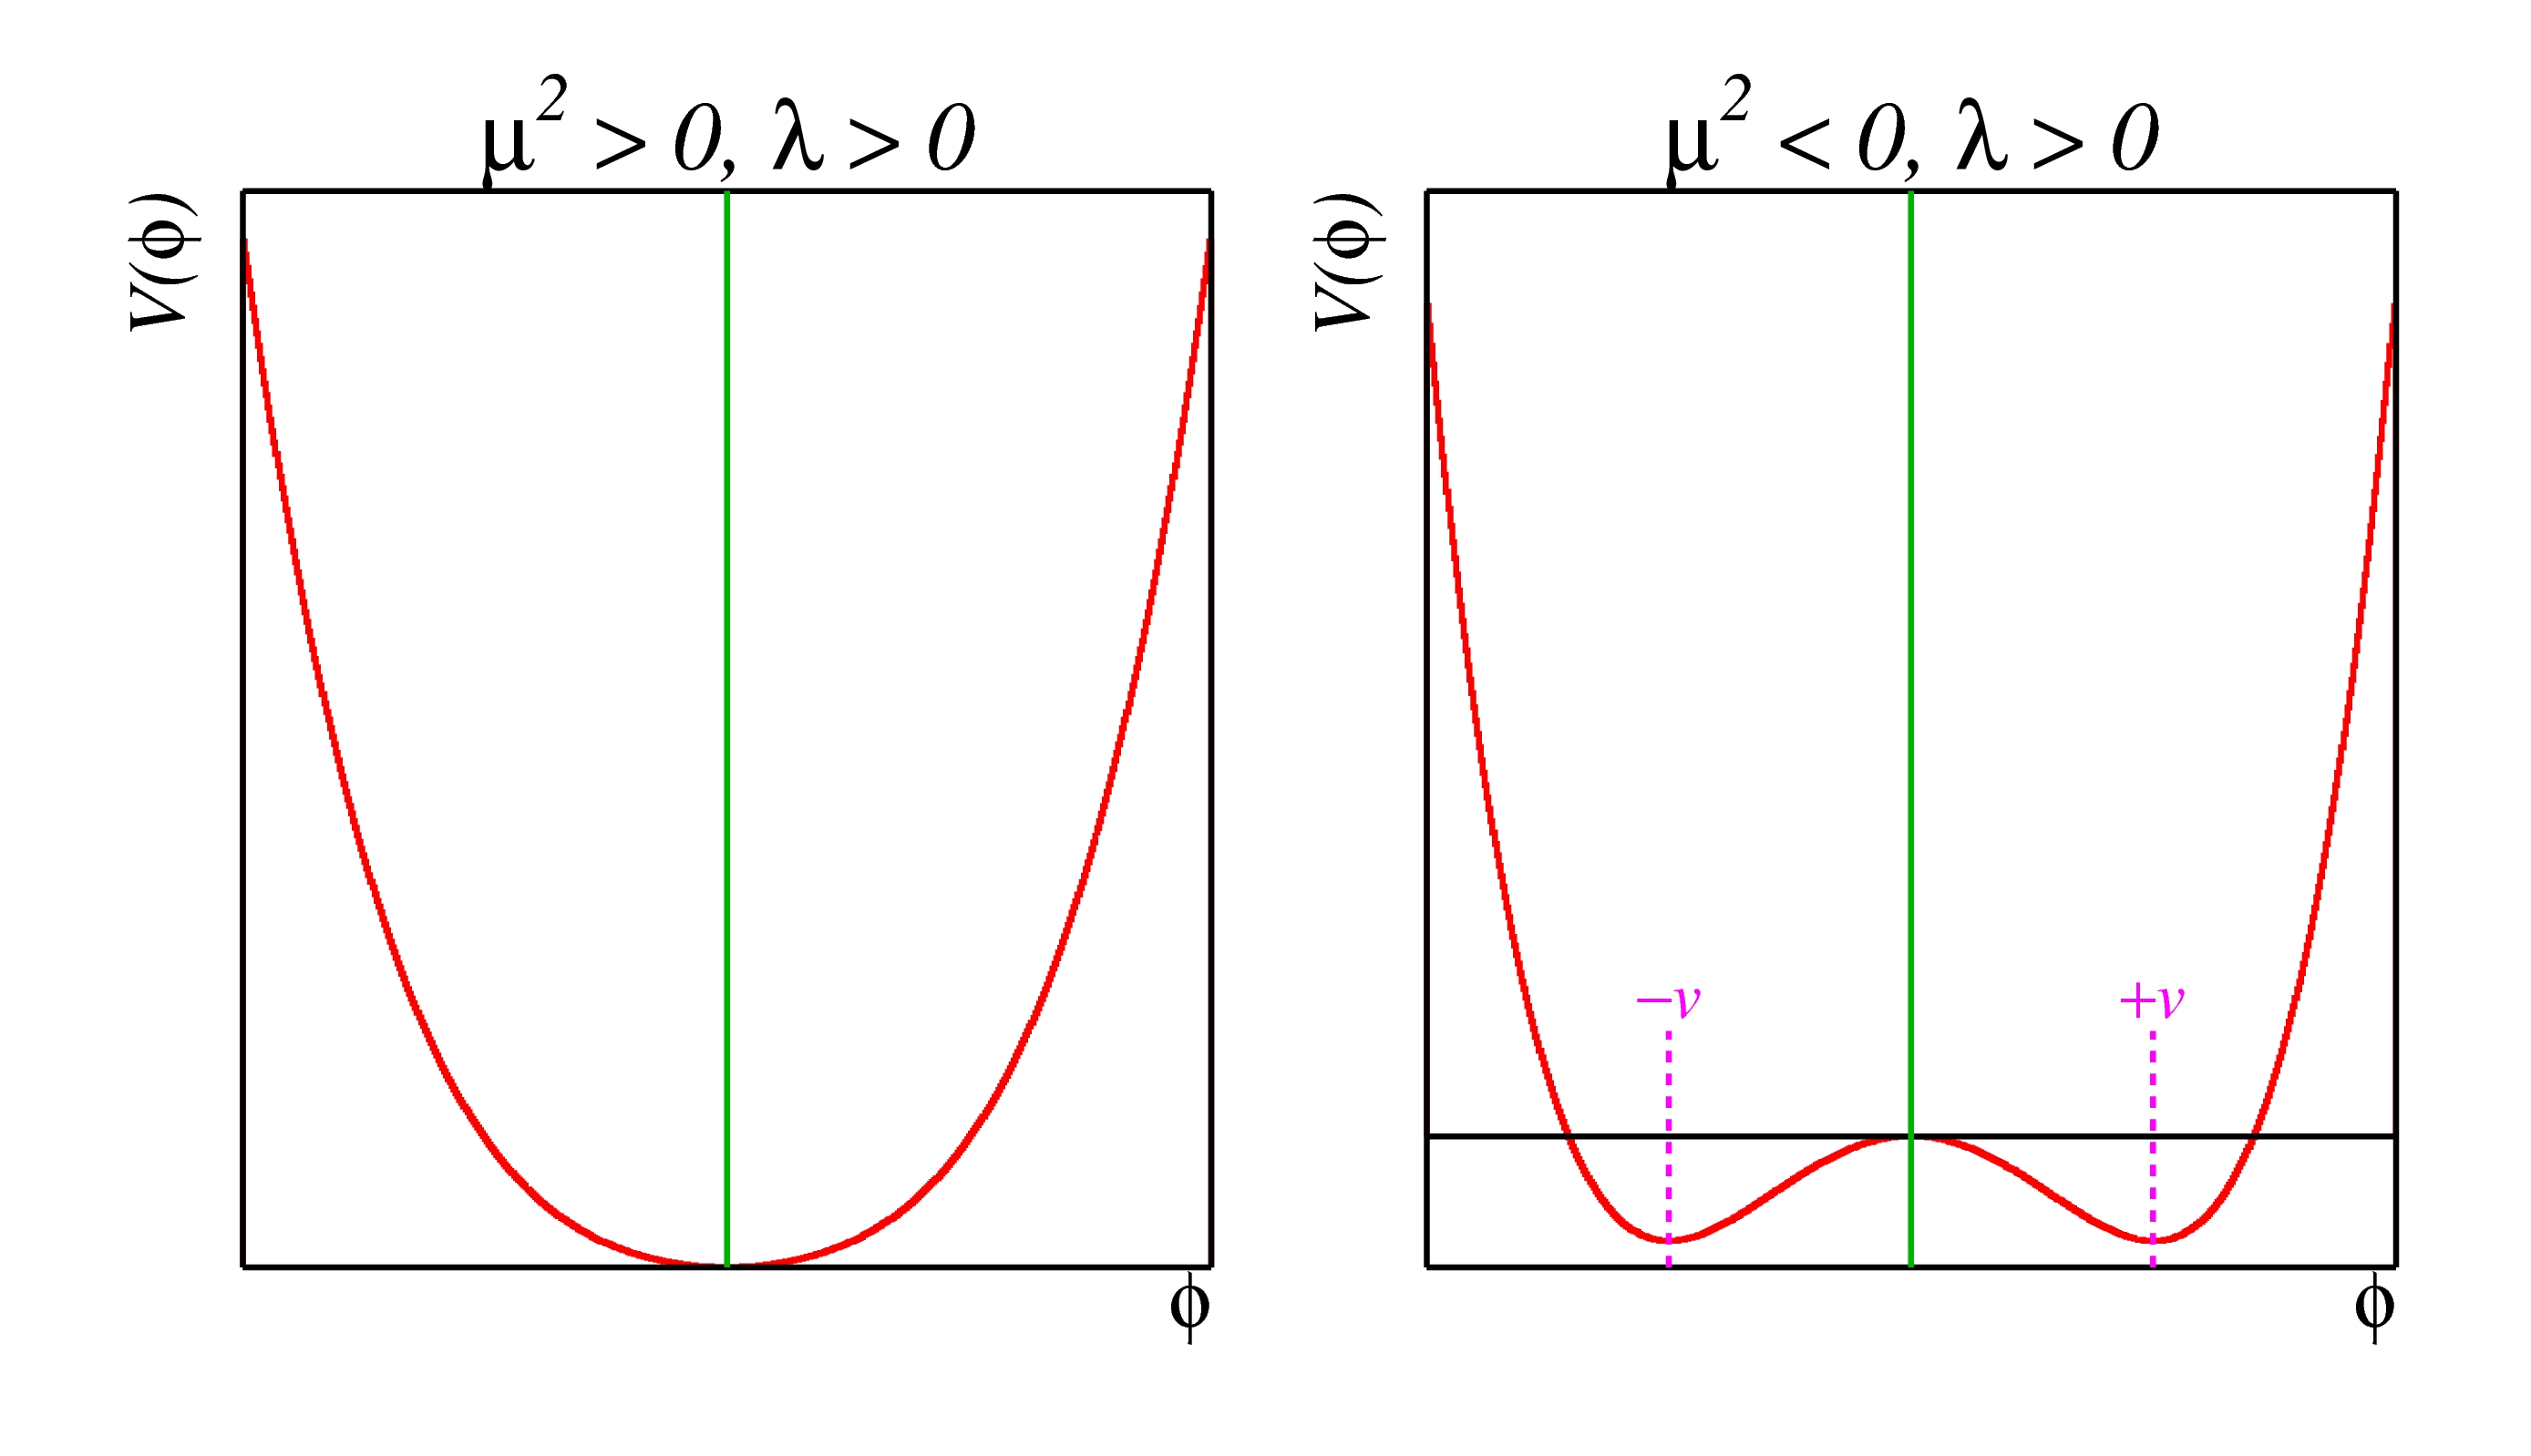
\includegraphics[scale=0.4]{hp2d}
\caption[SSB Potential form]{Shape of the potential $V(\phi)$ for $\lambda>0$ and: $\mu^2>0$ (left) and $\mu^2<0$ (right). The case $\mu^2<0$ corresponds to the potential suitable for introducing the SSB mechanism by choosing one of the two ground states which are connected via reflection symmetry. \cite{broken_symmetry}.}
\label{hp2d}
\end{figure}

In the case of a complex scalar field $\phi(x)$

\beqn\label{complex_scalar}
\phi(x)=\frac{1}{\sqrt{2}}(\phi_1 + i \phi_2)
\eeqn
\noindent the Lagrangian (invariant under global $U(1)$ transformations) is given by 
\beqn\label{higgs_potential}
\Lagr=(\partial_\mu\phi)^\dagger(\partial^\mu\phi) - V(\phi) , \qquad V(\phi)=\mu^2\phi^\dagger\phi + \lambda(\phi^\dagger\phi)^2
\eeqn

\noindent where an appropriate potential has been added in order to introduce the SSB.

As seen in Figure \ref{higgs_potential_plot}, the potential has now an infinite number of minima circularly distributed along the $\xi$-direction which makes possible the occurrence of the SSB by choosing an arbitrary ground state; for instance, $\xi=0$, \ie $\phi_1=v, \phi_2=0$

\begin{figure}[!h]
\centering
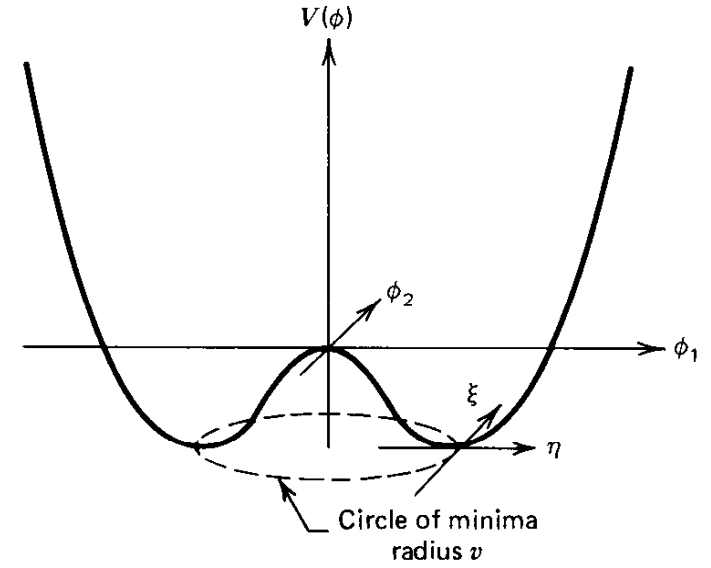
\includegraphics[scale=0.3]{higgs_potential_plot}
\caption[Potential for complex scalar field ]{Potential for complex scalar field. There is a circle of minima of radius \textit{v} along the $\xi$-direction\cite{halzen}.}
\label{higgs_potential_plot}
\end{figure}

\beqn
\phi_0=\frac{v}{\sqrt{2}}\exp(i\xi) \quad \xrightarrow[]{SSB} \quad \phi_0=\frac{v}{\sqrt{2}}
\eeqn

As usual, excitations over the ground state are studied by making an expansion about it; thus, the excitations can be parametrized as:
\beqn
\phi(x)=\frac{1}{\sqrt{2}}(v + \eta(x) + i\xi(x))
\eeqn

\noindent which when substituted into Eqn. \ref{higgs_potential} produces a Lagrangian in terms of the new fields $\eta$ and $\xi$

\beqn\label{lagr_complex_field}
\Lagr'=\frac{1}{2}(\partial_\mu\xi)^2 + \frac{1}{2}(\partial_\mu\eta)^2 + \mu^2\eta^2 - V(\phi_0) - \lambda v \eta(\eta^2+\xi^2) -  \frac{\lambda}{4}(\eta^2+\xi^2)^2
\eeqn

\noindent where the last two terms represent the interactions and self-interaction between the two fields $\eta$ and $\xi$. The particular feature of the SSB mechanism is revealed when looking to the first three  terms of $\Lagr'$. Before the SSB, only the massless $\phi$ field is present in the system; after the SSB there are two fields of which the $\eta$-field has acquired mass $m_\eta=\sqrt{-2\mu^2}$ while the $\xi$-field is still massless (see Figure \ref{higgs_hat}).\\  

\begin{figure}[!h]
\centering
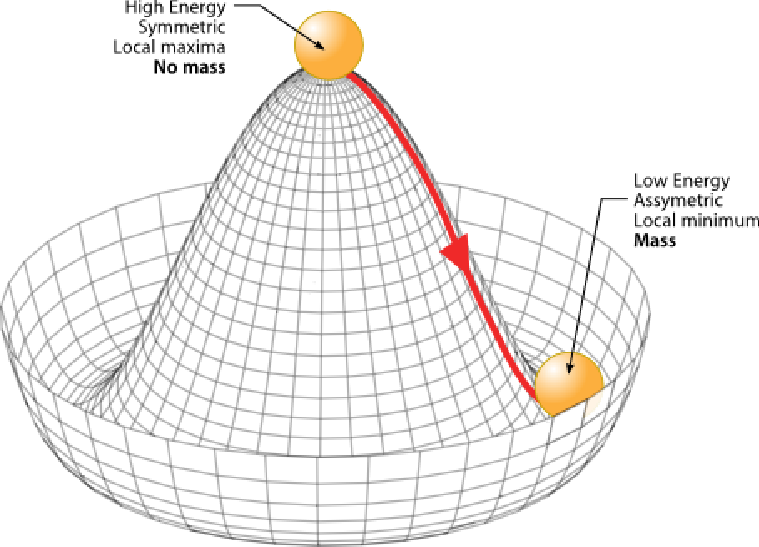
\includegraphics[width=0.48\textwidth]{higgs_hat}
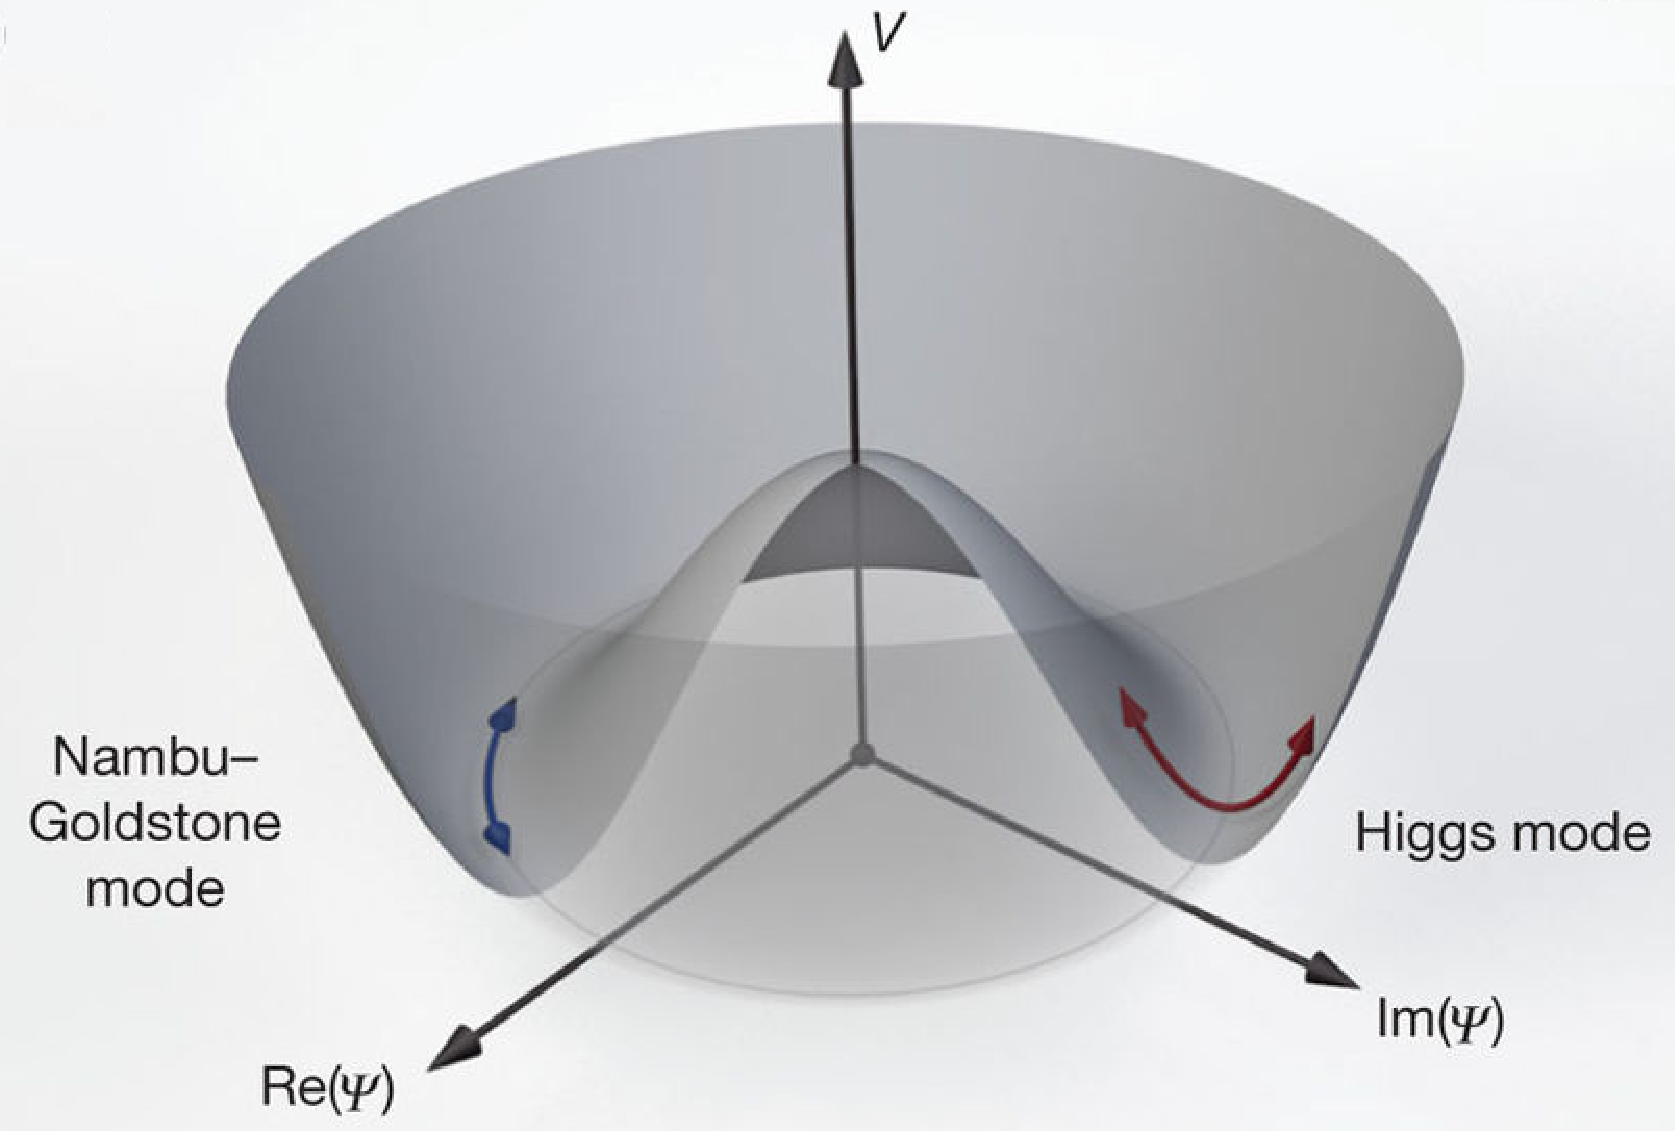
\includegraphics[width=0.5\textwidth]{goldstone_boson_mode}
\caption[SSB mechanism for complex scalar field]{SSB mechanism for a complex scalar field\cite{broken_symmetry,endres}.}
\label{higgs_hat}
\end{figure}

Thus, \textit {the SSB mechanism serves as a method to generate mass but as a side effect a massless field is introduced in the system}. This fact is known as the Goldstone theorem and states that a massless scalar field appears in the system for each continuous symmetry spontaneously broken. Another version of the Goldstone theorem states that \textit{``if a Lagrangian is invariant under a continuous symmetry group G, but the vacuum is only invariant under a subgroup $H\subset G$, then there must exist as many massless spin-0 particles (Nambu-Goldstone bosons) as broken generators.''}\cite{pich} The Nambu-Goldstone boson can be understood considering that the potential in the $\xi$-direction is flat so excitations in that direction are not energy consuming and thus represent a massless state.                   

\subsection{Higgs mechanism}

\noindent When the SSB mechanism is introduced in the formulation of the EWI in an attempt to generate the mass of the so far massless gauge bosons and fermions, an interesting effect is revealed. In order to keep the G symmetry group invariance and generate the mass of the EW gauge bosons, a G invariant Lagrangian density ($\Lagr_S$) has to be added to the non massive EWI Lagrangian (Eqn. \ref{nmewi_lagr})

\begin{align}
\Lagr_S    = &(D_\mu\phi)^\dagger(D^\mu\phi) - \mu^2\phi^\dagger\phi - \lambda(\phi^\dagger\phi)^2 , \qquad \lambda>0, \mu^2<0 \label{ls}\\
D_\mu\phi = &\left(i\partial_\mu - g\frac{\sigma_i}{2}W^i_\mu -
g'\frac{Y}{2}B_\mu\right)\phi
\end{align}

\noindent $\phi$ has to be an isospin doublet of complex scalar fields so it preserves the G invariance; thus $\phi$ can be defined as:

\beqn
\phi = \binom{\phi^+}{\phi^0} \equiv \frac{1}{\sqrt{2}}\binom{\phi_1 + i\phi_2}{\phi_3 + i\phi_4}.
\eeqn

The minima of the potential are defined by

\beqn
\phi^\dagger\phi=\frac{1}{2}(\phi_1^2 +\phi_2^2 +\phi_3^2 + \phi_1^4 )= -\frac{\mu^2}{2\lambda}.
\eeqn

The choice of the ground state is critical. By choosing a ground state, invariant under $U(1)_{em}$ gauge symmetry, the photon will remain massless and the $\wpm$ and $Z$ bosons masses will be generated which is exactly what is needed. In that sense, the best choice corresponds to a weak isospin doublet with $T_3=-1/2$, $Y_W=1$ and $Q=0$ which defines a ground state with $\phi_1=\phi_2=\phi_4$ and $\phi_3=v$:

\beqn\label{field_exp}
\phi_0\equiv\frac{1}{\sqrt{2}}\binom{0}{v}, \qquad v^2\equiv-\frac{\mu^2}{\lambda}.
\eeqn

\noindent where the vacuum expectation value $v$ is fixed by the Fermi coupling $G_F$ according to $v=(\sqrt{2}G_F)^{1/2}\approx 246$ GeV.

The G symmetry has been broken and three Nambu-Goldstone bosons will appear. The next step is to expand $\phi$ about the chosen ground state as:
\beqn
\phi(x) = \frac{1}{\sqrt{2}}\exp\left(\frac{i}{v}\sigma_i\theta^i(x)\right) \binom{0}{v+H(x)}\approx \frac{1}{\sqrt{2}}\binom{\theta_1(x) + i\theta_2(x)}{v + H(x) - i\theta_3(x)} 
\eeqn

\noindent to describe fluctuations from the ground state $\phi_0$. The fields $\theta_i(x)$ represent the Nambu-Goldstone bosons while $H(x)$ is known as \ti{Higgs field.} The fundamental feature of the parametrization used is that the dependence on the $\theta_i(x)$ fields is factored out in a global phase that can be eliminated by taking the physical \ti{unitary gauge} $\theta_i(x)=0$. Therefore the expansion about the ground state is given by:
\beqn\label{higgs_dublet}
\phi(x)\frac{1}{\sqrt{2}}\binom{0}{v+H(x)}
\eeqn

\noindent which when substituted into $\Lagr_S$ (Eqn. \ref{ls}) results in a Lagrangian containing the now massive three gauge bosons $\wpm, Z$, one massless gauge boson (photon) and the new Higgs field (H). The three degrees of freedom corresponding to the Nambu-Goldstone bosons are now integrated into the massive gauge bosons as their longitudinal polarizations which were not available when they were massless particles. The effect by which vector boson fields acquire mass after an spontaneous symmetry breaking, but without an explicit gauge invariance breaking is known as the \textit{Higgs mechanism}.

The mechanism was proposed by three independent groups: F.Englert and R.Brout in August 1964 \cite{englert}, P.Higgs in October 1964 \cite{higgs} and G.Guralnik, C.Hagen and T.Kibble in November 1964\cite{ghk}; however, its importance was not realized until S.Glashow\cite{glashow}, A.Salam\cite{salam} and S.Weinberg \cite{weinberg}, independently, proposed that electromagnetic and weak interactions are two manifestations of a more general interaction called \ti{electroweak interaction} in 1967.

\subsection{Masses of the gauge bosons}

The masses of the gauge bosons are extracted by evaluating the kinetic part of Lagrangian $\Lagr_S$ in the ground state (known also as the vacuum expectation value), \ie,

\beqn\label{gauge_masses}
\small
\left|\left(\partial_\mu - ig\frac{\sigma_i}{2}W^i_\mu -i\frac{g'}{2}B_\mu\right)\phi_0\right |^2= \left(\frac{1}{2}vg\right)^2W_\mu^+W^{-\mu} + \frac{1}{8}v^2(W_\mu^3,B_\mu)\binom{g^2 \quad -gg'}{-gg' \quad g'^2}\binom{W^{3\mu}}{B^\mu}
\eeqn

\noindent comparing with the typical mass term for a charged boson $M_W^2 W^+W^-$
\beqn
M_W=\frac{1}{2}vg.
\eeqn
The second term in the right side of the Eqn.\ref{gauge_masses} comprises the masses of the neutral bosons, but it needs to be written in terms of the gauge fields $Z_\mu$ and $A_\mu$ in order to be compared to the typical mass terms for neutral bosons, therefore using Eqn. \ref{neutral_bosons}
\begin{align}
\frac{1}{8}v^2[g^2(W_\mu^3)^2-2gg'W_\mu^3B^\mu + g'^2B_\mu^2]=&\frac{1}{8}v^2[ g W^3_\mu - g'B_\mu]^2 + 0[g'W^3_\mu + gB_\mu]^2\\
                                                             =&\frac{1}{8}v^2[\sqrt{g^2+g'^2}Z_\mu]^2 + 0[\sqrt{g^2+g'^2}A_\mu]^2\nonumber                                                             
\end{align}

\noindent and then

\beqn
M_Z= \frac{1}{2}v\sqrt{g^2+g'^2}, \qquad M_A=0 
\eeqn

\subsection{Masses of the fermions}
The lepton mass terms can be generated by introducing a gauge invariant Lagrangian term describing the Yukawa coupling between the lepton field and the Higgs field
\beqn\label{lyl}
\Lagr_{Yl}=-G_l\left[(\bar{\nu_l}, \bar{l})_L\binom{\phi^+}{\phi^0}l_R + \bar{l}_R(\phi^-,\bar{\phi}^0)\binom{\nu_l}{l}_L\right], \qquad l=e,\mu,\tau.
\eeqn

 After the SSB and replacing the usual field expansion about the ground state (Eqn.\ref{field_exp}) into $\Lagr_{Yl}$, the mass term arises
\beqn\label{lyl2}
\Lagr_{Yl}=-m_l(\bar{l}_Ll_R + \bar{l}_R{l}_L) -\frac{m_l}{v}(\bar{l}_Ll_R + \bar{l}_R{l}_L)H= -m_l \bar{l}l\left(1+ \frac{H}{v}\right)                   
\eeqn
\beqn
m_l=\frac{G_l}{\sqrt{2}}v
\eeqn
\noindent where the additional term represents the lepton-Higgs interaction. The quark masses are generated in a similar way as lepton masses but for the upper member of the quark doublet a different Higgs doublet is needed:
\beqn
\phi_c=-i\sigma_2\phi* = \binom{-\bar{\phi}^0}{\phi^-}.
\eeqn

Additionally, given that the quark isospin doublets are not constructed in terms of the mass eigenstates but in terms of the flavor eigenstates, as shown in Table\ref{T3Y}, the coupling parameters will be related to the CKM matrix elements; thus the quark Lagrangian is given by:   

\beqn\label{lyq}
\Lagr_{Yq}=-G_d^{i,j}(\bar{u_i},\bar{d'_i})_L\binom{\phi^+}{\phi^0}d_{jR} - G_u^{i,j}(\bar{u_i},\bar{d'_i})_L\binom{-\bar{\phi^0}}{\phi^-}u_{jR} + h.c. 
\eeqn

\noindent with i,j=1,2,3. After SSB and expansion about the ground state, the diagonal form of $\Lagr_{Yq}$ is:
\beqn\label{lyq2}
\Lagr_{Yq}=-m_d^i\bar{d_i}d_i\left(1 +\frac{H}{v}\right) - m_u^i\bar{u_i}u_i\left(1 +\frac{H}{v}\right)
\eeqn

Fermion masses depend on arbitrary couplings $G_l$ and $G_{u,d}$ and are not predicted by the theory.  

\subsection{The Higgs field}

After the characterization of the fermions and gauge bosons as well as their interactions, it is necessary to characterize the Higgs field itself. The Lagrangian $\Lagr_S$ in Eqn. \ref{ls} written in terms of the gauge bosons is given by
\beqn
\Lagr_S= \frac{1}{4}\lambda v^4 + \Lagr_H +\Lagr_{HV}
\eeqn
\beqn\label{lh}
\Lagr_H= \frac{1}{2}\partial_\mu H\partial^\mu H -  \frac{1}{2}m_H^2 H^2 - \frac{1}{2v}m_H^2 H^3 -  \frac{1}{8v^2}m_H^2 H^4
\eeqn
\beqn\label{lhV}
\Lagr_{HV}= m_H^2W_\mu^+W^{\mu-}\left(1+ \frac{2}{v}H +  \frac{2}{v^2}H^2 \right) + \frac{1}{2}m_Z^2Z_\mu Z^\mu\left(1+ \frac{2}{v}H +  \frac{2}{v^2}H^2 \right) 
\eeqn
The mass of the Higgs boson is deduced as usual from the mass term in the Lagrangian resulting in:
\beqn
m_H=\sqrt{-2\mu^2}=\sqrt{2\lambda}v
\eeqn
\noindent however, it is not predicted by the theory either. The experimental efforts to find the Higgs boson, carried out by the \ti{Compact Muon Solenoid (CMS)} experiment and the \ti{A Toroidal LHC AppartuS (ATLAS)} experiments at the \ti{Large Hadron Collider(LHC)}, gave great results by July of 2012 when the discovery of a new particle compatible with the Higgs boson predicted by the electroweak theory\cite{hcms,hatlas} was announced. Although at the announcement time there were some reservations about calling the new particle the \ti{Higgs boson}, today this name is widely accepted. The Higgs mass measurement, reported by both experiments\cite{hmass}, is in Table \ref{higgs_prop}. 
\begin{center}
\begin{table}[h]
\centering
\scriptsize
\begin{tabular}{lc}\hline
Property         & Value  \\ \hline
Electric charge  & 0      \\
Color charge    & 0      \\
Spin             & 0      \\
Weak isospin     & -1/2    \\
Weak hypercharge & 1      \\
Parity           & 1      \\\hline
Mass (GeV/c$^2$) & 125.09$\pm$0.21 (stat.)$\pm$0.11 (syst.)\\\hline
\end{tabular}
\caption[Higgs boson properties.]{Higgs boson properties. Higgs mass is not predicted by the theory and the value here corresponds to the experimental measurement.}\label{higgs_prop}
\end{table}
\end{center}

\subsection{Production of Higgs bosons at LHC}

At the LHC, Higgs bosons are produced as a result of the collision of two counter-rotating protons beams. A detailed description of the LHC machine will be presented in chapter \ref{ch:cms}.% \ti{The total cross section} is a parameter that quantifies the number of \pp collisions that happen when a number of protons are fired at each other. Different results can be obtained after a \pp collision and for each one the \ti{cross section} is defined as the number of \pp collisions that conclude in that particular result with respect to the number of protons fired at each other.
\begin{figure}[!h]
\centering
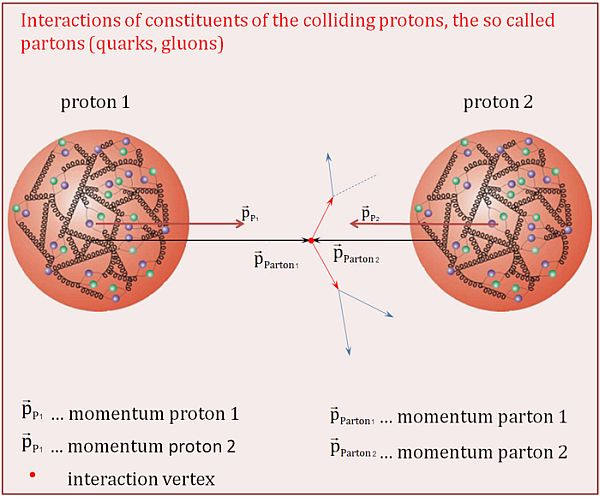
\includegraphics[scale=0.55]{proton_proton}
\caption[Proton-Proton collision]{Proton-proton collision. Protons are composed of 3 valence quarks, a sea of quarks and gluons; therefore in a proton-proton collision, quarks and gluons are those who collide. \cite{pp_coll}.}
\label{pp_collision}
\end{figure}

Protons are composed of quarks and these quarks are bound by gluons; however, what is commonly called the quark content of the proton makes reference to the valence quarks. In fact, a proton is not just a rigid entity with three balls in it all tied up with springs, but the gluons exchanged by the valence quarks tend to split spontaneously into quark-antiquark pairs or more gluons, creating \ti{sea of quarks and gluons} as represented in Figure \ref{pp_collision}.

In a proton-proton (\pp) collision, the proton's constituents, quarks and gluons, are those that collide. The \pp cross section depends on the momentum of the colliding particles, reason for which it is needed to know how the momentum is distributed inside the proton. Quarks and gluons are known as partons, hence, the functions that describe how the proton momentum is distributed among partons inside it are called \ti{parton distribution functions (PDFs)}; PDFs are determined from experimental data obtained in experiments where the internal structure of hadrons is tested.

In addition, in physics, a common approach to study complex systems consists of starting with a simpler version of them, for which a well known description is available, and adding an additional \ti{perturbation} which represents a small deviation from the known behavior. If the perturbation is small enough, the physical quantities associated with the perturbed system are expressed as a series of corrections to those of the simpler system. The perturbation series corresponds to an expansion in power series of a small parameter, therefore, the more terms are considered in the series (the higher order in the perturbation series), the more precise is the the description of the complex system. If the perturbation does not get progressively smaller, the strategy cannot be applied and new methods have to be employed. 

High energy systems, like the Higgs production at LHC explored in this thesis, usually can be treated perturbatively with the expansion made in terms of the coupling constants. The overview presented here will be oriented specifically to the Higgs boson production mechanisms in \pp collisions at LHC.

\begin{figure}[!h]
\centering
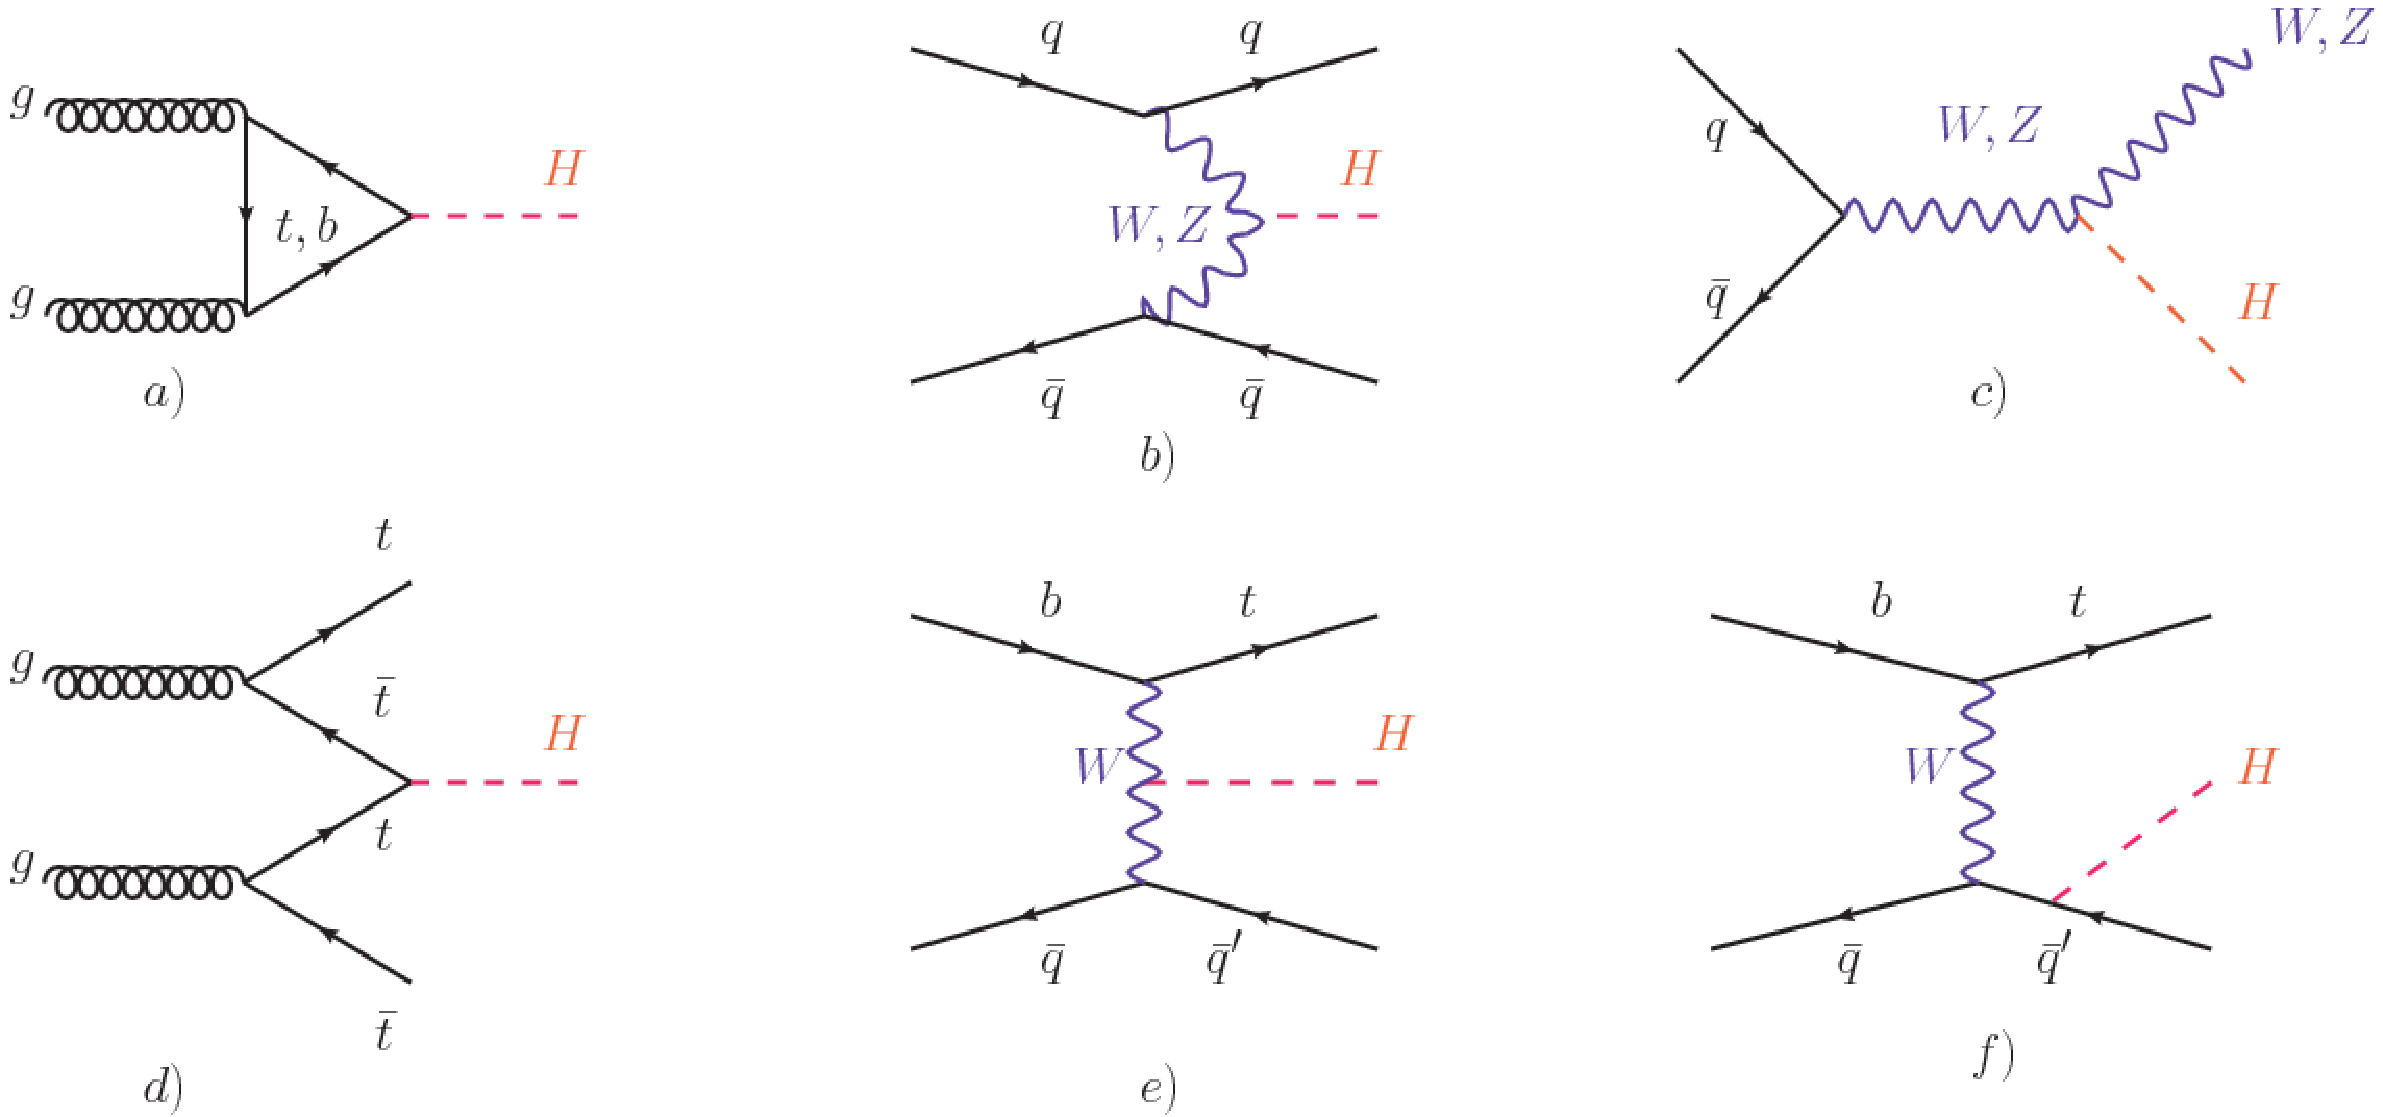
\includegraphics[scale=0.3]{higgs_prod}
\caption[Higgs boson production mechanism Feynman diagrams]{Main Higgs boson production mechanism Feynman diagrams. a. gluon-gluon fusion, b. vector boson fusion (VBF), c. Higgs-strahlung, d. Associated production with a top or bottom quark pair, e-f. associated production with a single top quark.}
\label{higgs_prod}
\end{figure}

Figure \ref{higgs_prod} shows the Feynman diagrams for the leading order (first order) Higgs production processes at LHC, while the cross section for Higgs production as a function of the center of mass-energy ($\sqrt{s}$) for \pp collisions is showed in Figure \ref{hcs_br} left. The tags NLO (next to leading order), NNLO (next to next to leading order) and N3LO (next to next to next to leading order) make reference to the order at which the perturbation series have been considered while the tags QCD and EW correspond to the strong and electroweak coupling constants respectively.
%% Table \ref{hxsec} present the cross sections for $m_H=125GeV/c^2$.
%% \begin{center}
%% \begin{table}[h]
%% \centering
%% \begin{tabular}{lllllll}\hline
%% $\sqrt{s}$(TeV) &\multicolumn{6}{l}{Production cross section (in pb) for $m_H$ = 125 GeV/c$^2$}\\\hline
%%                 & ggF          & VBF          & WH           & ZH           & $t\bar{t}H$           & total \\\hline
%% 7               & $16.9\pm5\%$ & $1.24\pm2\%$ & $0.58\pm3\%$ & $0.34\pm4\%$ & $0.09^{+8\%}_{-14\%}$ & 19.1  \\
%% 8               & $21.4\pm5\%$ & $1.60\pm2\%$ & $0.70\pm3\%$ & $0.42\pm5\%$ & $0.13^{+8\%}_{-13\%}$ & 24.2  \\
%% 13              & $48.6\pm5\%$ & $3.78\pm2\%$ & $1.37\pm2\%$ & $0.88\pm5\%$ & $0.50^{+9\%}_{-13\%}$ & 55.1  \\
%% 14              & $54.7\pm5\%$ & $4.28\pm2\%$ & $1.51\pm2\%$ & $0.99\pm5\%$ & $0.60^{+9\%}_{-13\%}$ & 62.1  \\\hline
%% \end{tabular}
%% \caption[The SM Higgs boson production cross sections for $m_H = 125 GeV/c^2$.]{The SM Higgs boson production cross sections for $m_H = 125 GeV/c^2$.in \pp collisions as a function of
%% the center of mass energy, $\sqrt{s}$. The predictions for the ggF channel at the LHC include the latest N3LO results leading to reduced theoretical uncertainties by a factor around 2 compared to the N2LO results.\cite{pdg}}\label{hxsec}
%% \end{table}
%% \end{center}

\begin{figure}[!h]
\centering
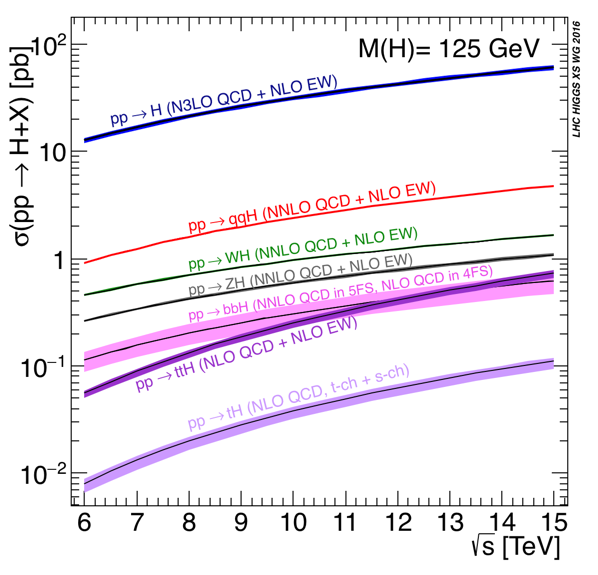
\includegraphics[width=0.40\textwidth]{higgs_prod_plot}
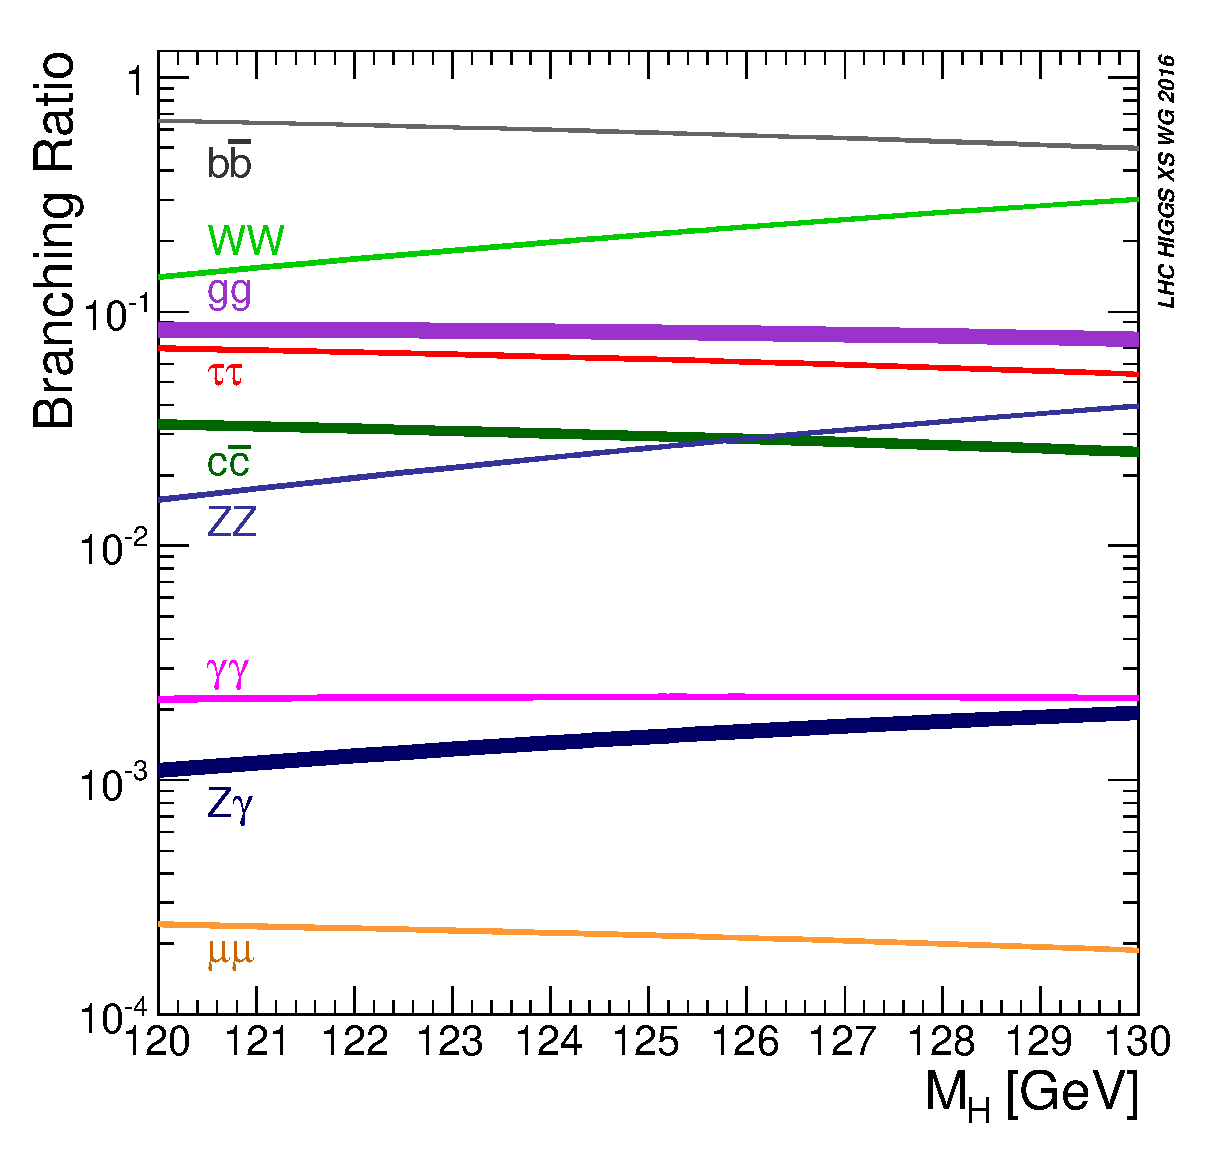
\includegraphics[width=0.40\textwidth]{higgsbr}
\caption[Higgs boson production cross section and decay branching ratios]{Higgs boson production cross sections (left) and decay branching ratios (right) for the main mechanisms. The VBF is indicated as qqH\cite{hcswg}.}
\label{hcs_br}
\end{figure}

%As shown in Eqns \ref{lyl}, \ref{lyq} and \ref{lhV}, the strength of the Higgs-fermion interaction is proportional to the fermion mass while the strength of the Higgs-gauge boson interaction is proportional to the square of the gauge boson mass, which implies that the Higgs production and decay mechanisms are dominated by couplings $H-(W,Z,t,b,\tau)$. 

The main production mechanism is the gluon fusion (Figure \ref{higgs_prod}a and $pp\to H$ in Figure \ref{hcs_br}) given that gluons carry the highest fraction of momentum of the protons in \pp colliders. Since the Higgs boson does not couple to gluons, the mechanism proceeds through the exchange of a virtual top-quark loop. Note that in this process the Higgs boson is produced alone, turning out to be problematic for some Higgs decays, because such absence of anything produced in association with the Higgs represent a trouble for triggering, however, this mechanism is experimentally clean when combined with the two-photon or the four-lepton decay channels (see Section \ref{sec:decays}). 

Vector boson fusion (Figure \ref{higgs_prod}b and $pp\to qqH$ in Figure \ref{hcs_br}) has the second largest production cross section. The scattering of two fermions is mediated by a weak gauge boson which later emits a Higgs boson. In the final state, the two fermions tend to be located in the central region of the detector; this kind of features are generally used as a signature when analyzing the datasets provided by the experiments\footnote{More details about how to identify events of interest in this analysis will be given in chapter \ref{ch:analysis}.}. 

The next production mechanism is Higgs-strahlung (Figure \ref{higgs_prod}c and $pp\to WH, pp\to ZH$ in Figure \ref{hcs_br}) where two fermions annihilate to form a weak gauge boson. If the initial fermions have enough energy, the emergent boson might emit a Higgs boson.

The associated production with a top or bottom quark pair and the associated production with a single top quark (Figure \ref{higgs_prod}d-f and $pp\to bbH, pp\to \ttH, pp\to tH$ in Figure \ref{hcs_br}) have a smaller cross section than the main three mechanisms above, but they provide a good opportunity to test the Higgs-top coupling. The analysis reported in this thesis is developed using these production mechanisms. A detailed description of the \tH mechanism will be given in Section \ref{sec:thq}.  

\subsection{Higgs boson decay channels}\label{sec:decays}

When a particle can decay through several modes, also known as channels, the probability of decaying through a given channel is quantified by the \ti{branching ratio (BR)} of the decay channel; thus, the BR is defined as the ratio of number of decays going through that given channel to the total number of decays. In regard to the Higgs boson decay, the BR can be predicted with accuracy once the Higgs mass is known \cite{riley, denner}. In Figure \ref{hcs_br} right, a plot of the BR as a function of the Higgs mass is presented; the largest predicted BR corresponds to the $\bbbar$ pair decay channel (see Table \ref{hdbr}) given that it is the heaviest particle pair whose on-shell \footnote{In general, on-shell or real particles are those which satisfy the energy-momentum relation ($E^2-|\vec{p}|^2c^2= m^2c^4$); off-shell or virtual particles does not satisfy it which is possible under the uncertainty principle of quantum mechanics. Usually, virtual particles correspond to internal propagators in Feynman diagrams.} production is kinematically allowed in the decay.

\begin{center}
\begin{table}[h]
\centering
\begin{tabular}{lll}\hline
Decay channel       & Branching ratio   & Rel. uncertainty\\\hline
$H\to b\bar{b}$     & $5.84\times10^{-1}$ & $+3.2\%-3.3\%$\\
$H\to W^+W^-$       & $2.14\times10^{-1}$ & $+4.3\%-4.2\%$\\
$H\to\tau^+\tau^-$  & $6.27\times10^{-2}$ & $+5.7\%-5.7\%$\\
$H\to ZZ$           & $2.62\times10^{-2}$ & $+4.3\%-4.1\%$\\
$H\to \gamma\gamma$ & $2.27\times10^{-3}$ & $+5.0\%-4.9\%$\\
$H\to Z\gamma$      & $1.53\times10^{-3}$ & $+9.0\%-8.9\%$\\
$H\to\mu^+\mu^-$    & $2.18\times10^{-4}$ & $+6.0\%-5.9\%$\\\hline
\end{tabular}
\caption[Predicted branching ratios for a SM Higgs boson with $m_H = 125$ GeV/c$^2$.]{Predicted branching ratios and the relative uncertainty for some decay channels of a SM Higgs boson with $m_H = 125$GeV/c$^2$ \cite{pdg}; the uncertainties are driven by theoretical uncertainties for the different Higgs boson partial widths and by parametric uncertainties associated to the strong coupling and the masses of the quarks which are the input parameters. Further details on these calculations can be found in Reference \cite{florian}}\label{hdbr}
\end{table}
\end{center}

Decays to other lepton and quark pairs, like electron, strange, up, and down quark pairs not listed in the table, are also possible but their likelihood is too small to measure since they are very lightweight, hence, their interaction with the Higgs boson is very weak. On other hand, the decay to top quark pairs is heavily suppressed due to the top quark mass ($\approx 173$ GeV/c$^2$).

Decays to gluons proceed indirectly through a virtual top quark loop while the decays to photons proceed through a virtual W boson loop, therefore, their branching ratio is smaller compared to direct interaction decays. Same is true for the decay to a photon and a Z boson.

In the case of decays to pairs of W and Z bosons, the decay proceed with one of the bosons being on-shell and the other being off-shell. The likelihood of the process diminish depending on how far off-shell are the virtual particles involved, hence, the branching ratio for W boson pairs is bigger that for Z boson pairs since Z boson mass is bigger that W boson mass.

Note that the decay to a pair of virtual top quarks is possible, but the probability is way too small. 

\section{Experimental status of the anomalous Higgs-fermion coupling}

\begin{figure}[h!]
\centering
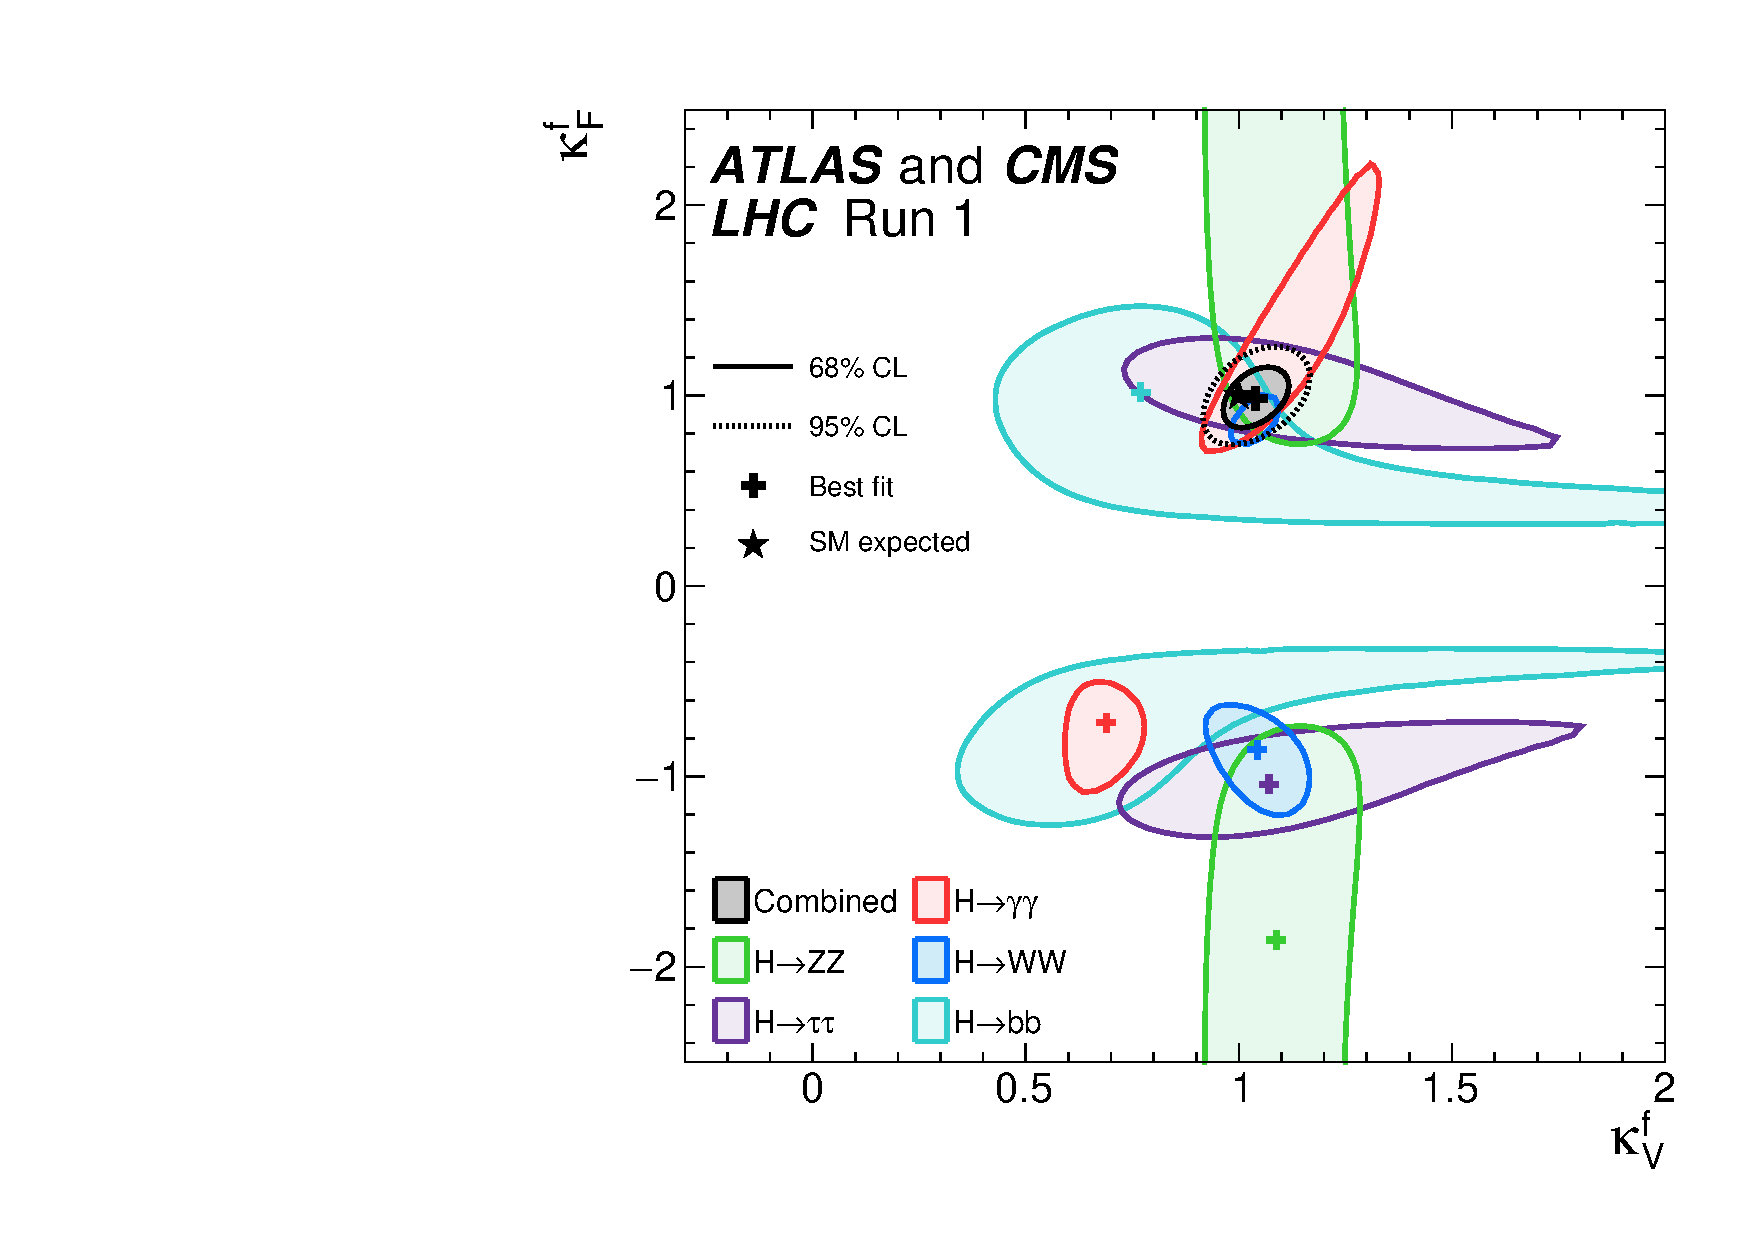
\includegraphics[scale=0.5]{kt_kv}
\caption[Two dimensional $\kappa_t$-$\kappa_V$ plot of the coupling modifiers. ATLAS and CMS combination.]{Combination of the  ATLAS and CMS fits for coupling modifiers $\kappa_t$-$\kappa_V$; also shown the individual decay channels combination and their global combination. No assumptions have been made on the sign of the coupling modifiers\cite{comb_ht_couplings}.} 
\label{fig:kt_kv}
\end{figure}
 
ATLAS and CMS have performed analyses of the anomalous H-f coupling by making likelihood scans for the two coupling modifiers, $\kappa_t$ and $\kappa_V$, under the assumption that $\kappa_Z=\kappa_W \equiv \kappa_V$ and $\kappa_t=\kappa_\tau=\kappa_b \equiv\kappa_f$. Figure \ref{fig:kt_kv} shows the result of the combination of ATLAS and CMS fits; also the individual decay channels combination and the global combination results are shown.

Note that from this plot there is limited information on the sign of the coupling  since most of the regions are sign-symmetric in $\kappa_F$; also, the only information available about the sign of the coupling comes from decays rather than production. 

While all the channels are compatible for positive values of the modifiers, for negative values of $\kappa_t$ there is no compatibility. The best fit for individual channels is compatible with negative values of $\kappa_t$ except for the $H\to bb$ channel which is expected to be the most sensitive channel; therefore, the best fit for the global fit yields $\kappa_t\geq0$. Thus, the anomalous H-t coupling cannot be excluded completely. That is what motivates to look at tHq, which can help with both of those.




%______________________ tHq ______________________
\section{Associated production of a Higgs boson and a single top quark}\label{sec:thq}

\begin{figure}[h!]
\centering
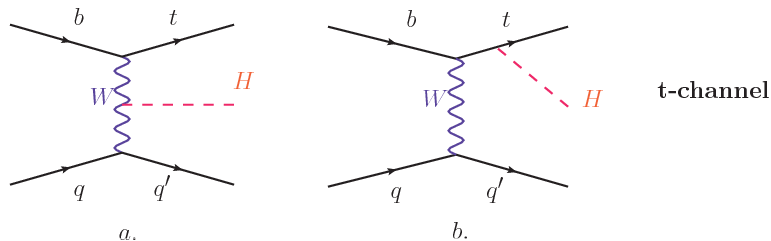
\includegraphics[scale=0.4]{thq_prod}\\
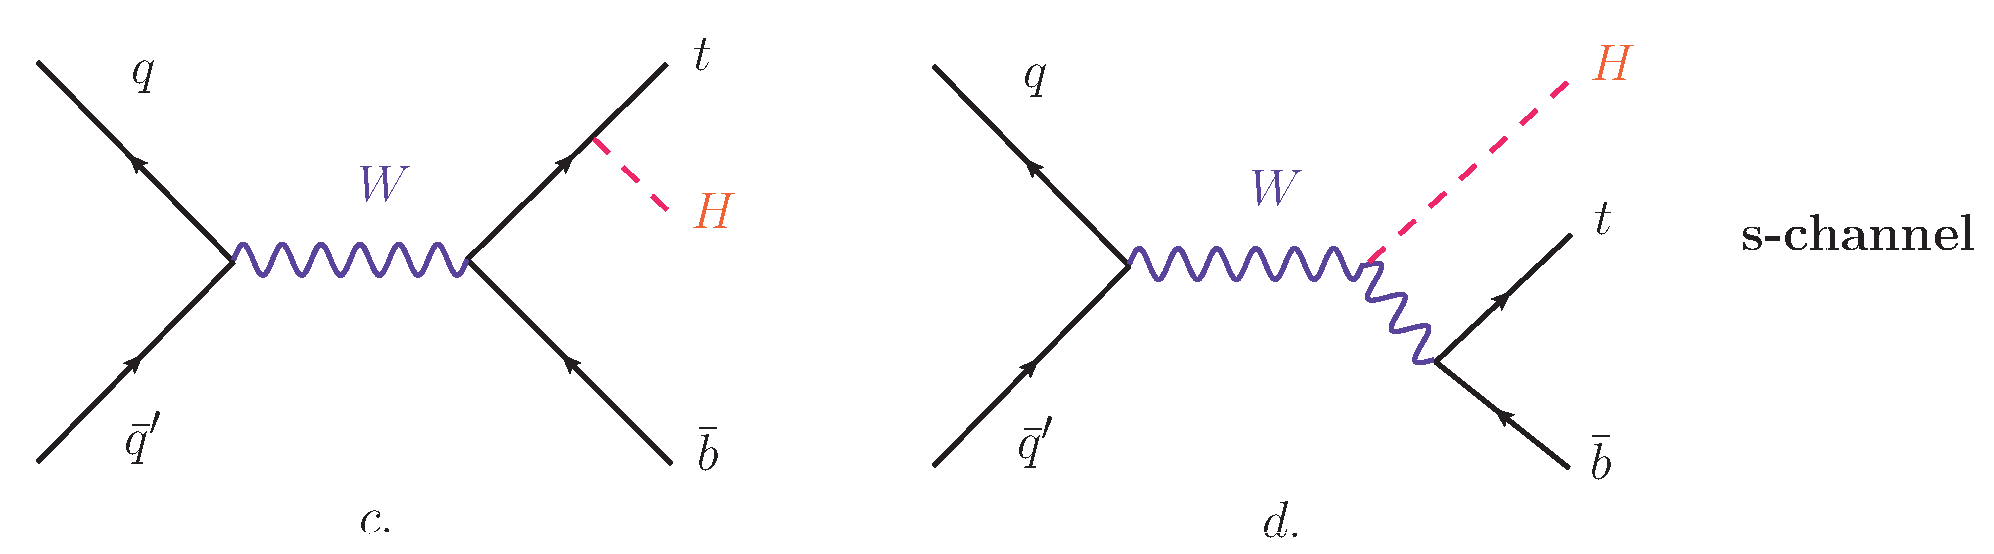
\includegraphics[scale=0.4]{thb_prod}\\
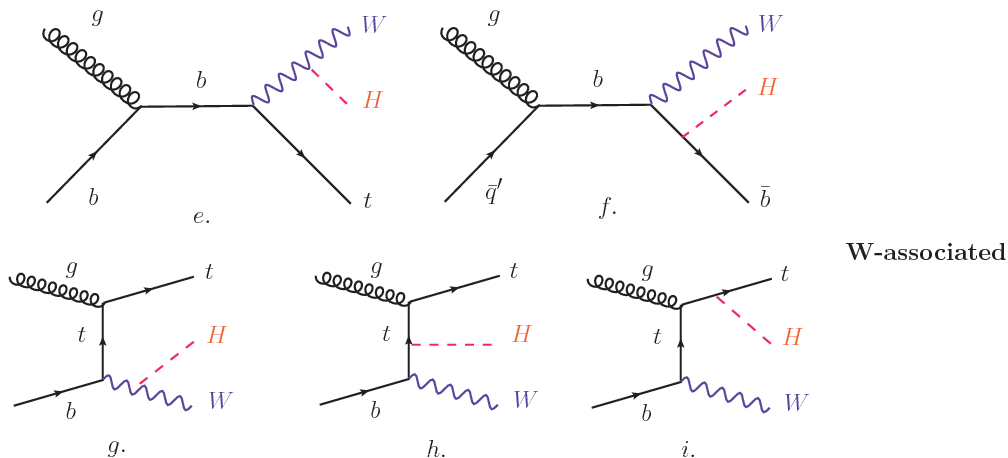
\includegraphics[scale=0.4]{thW_prod}\\
\caption[Higgs boson production in association with a top quark mechanism Feynman diagrams]{Associated Higgs boson production with a top quark mechanism Feynman diagrams. a.,b. t-channel (\tHq), c.,d. s-channel ($tHb$), e-i. W-associated.}
\label{fig:th_prod}
\end{figure}

The production of Higgs boson in association with a top quark has been extensively studied \cite{maltoni1, biswas, farina,tait, maltoni2}. While measurements of the main Higgs production mechanisms rates are sensitive to the strength of the Higgs coupling to W boson or top quark, they are not sensitive to the relative sign between the two couplings. In this thesis, the Higgs boson production mechanism explored is the associated production with a single top quark (\tH) which offers sensitivity to the relative sign of the Higgs couplings to W boson and to top quark. The description given here is based on Reference \cite{farina}

A process where two incoming particles interact and produce a final state with two particles can proceed in three called channels (see, for instance, Figure \ref{fig:th_prod} omitting the red line). The t-channel represents processes where an intermediate particle is emitted by one of the incoming particles and absorbed by the other. The s-channel represents processes where the two incoming particles merge into an intermediate particle which eventually will split into the particles in the final state. The third channel, u-channel, is similar to the t-channel but the two outgoing particles interchange their roles. These three channels are connected to the so-called Mandelstam variables 
%{\setlength{\mathindent}{0cm}
\begin{align}
&s =(p_1 +p_2)^2 =(p_1' + p_2')^2 \to{\small \textrm{ square of the center mass-energy}}.\\
&t =(p_1 -p_1')^2 =(p_2' -p_2)^2 \to{\small \textrm{ square of the four-momentum transfer}}.\\
&u =(p_1 -p_2')^2 =(p_1' - p_2)^2 \to{\small \textrm{ square of the crossed four-momentum transfer}}.\\
&s+t+u = m_1^2 + m_2^2 + m_1^{'2} +  m_2^{'2}
\end{align}
%}
\noindent which relate the momentum, energy and the angles of the incoming and outgoing particles in an scattering process of two particles to two particles. The importance of the Mandelstam variables reside in that they form a minimum set of variables needed to describe the kinematics of this scattering process; they are Lorentz invariant which makes them very useful when doing calculations.      

The \tH production, where Higgs boson can be radiated either from the top quark or from the W boson, is represented by the leading order Feynman diagrams in Figure \ref{fig:th_prod}. The cross section for the \tH process is calculated, as usual, summing over the contributions from the different Feynman diagrams; therefore it depends on the interference between the contributions. In the SM, the interference for t-channel (\tHq process)  and W-associated (\tHW process) production is destructive \cite{maltoni1} resulting in the small cross sections presented in Table \ref{tab:th_xsec}. 

\begin{center}
\begin{table}[h]
\centering
\begin{tabular}{lll}\hline
tH production channel       & Cross section (fb)      \\\hline
t-channel $(pp \to tHq)$    & $70.79^{+2.99}_{-4.80}$ \\
W-associated $(pp \to tHW)$ & $15.61^{+0.83}_{-1.04}$ \\
s-channel$(pp \to tHb)$     & $ 2.87^{+0.09}_{-0.08}$ \\\hline
\end{tabular}
\caption[Predicted SM cross sections for \tH production at $\sqrt{s}=13$ TeV.]{Predicted SM cross sections for \tH production at $\sqrt{s}=13$ TeV \cite{thqw_xsec, thb_xsec}.}\label{tab:th_xsec}
\end{table}
\end{center}

The s-channel contribution can be neglected. It will be shown that a deviation from the SM destructive interference would result in an enhancement of the \tH cross section compared to that in SM, which could be used to get information about the sign of the Higgs-top coupling \cite{farina,tait}. In order to describe \tH production processes, Feynman diagram \ref{fig:th_prod}b will be considered; there, the W boson is radiated by a quark in the proton and eventually it will interact with the b quark. In the high energy regime, the effective W approximation \cite{dawson} is used to describe the process as the emission of an approximately on-shell W and its hard scattering with the b quark; \ie $Wb \to th$. The scattering amplitude for the process is given by

\begin{equation} \label{s_amp}
\mathcal{A}= \frac{g}{\sqrt{2}}\left[(\kappa_t-\kappa_V)\frac{m_t\sqrt{s}}{m_Wv}\,A\left(\frac{t}{s},\varphi; \xi_{t},\xi_{b}\right)+\left(\kappa_V\,\frac{2m_W}{v}\frac{s}{t}+(2\kappa_t-\kappa_V)\,\frac{m_t^{2}}{m_Wv}\right)\,B\left(\frac{t}{s},\varphi; \xi_{t},\xi_{b}\right)\right]\,,
\end{equation}

\noindent where $\kappa_V\equiv g_{HVV}/g_{HVV}^{SM}$ and $\kappa_t\equiv g_{Ht}/g_{Ht}^{SM}=y_t/y_t^{SM}$ are scaling factors that quantify possible deviations of the couplings from the SM values, Higgs-Vector boson (H-W) and Higgs-top (H-t) respectively, from the SM couplings; $s=(p_{W}+p_{b})^{2}$, $t=(p_{W}-p_{H})^{2}$, $\varphi$ is the Higgs azimuthal angle around the $z$ axis taken parallel to the direction of motion of the incoming W; A and B are functions describing the weak interaction in terms of the chiral states ($\xi_{t},\xi_{b}$) of the quarks $b$ and $t$. Terms that vanish in the high energy limit have been neglected as well as the Higgs and \textit{b} quark masses\footnote{A detailed explanation of the structure and approximations used to derive $\mathcal{A}$ can be found in Reference \cite{farina}}.\\        

The scattering amplitude grows with energy like $\sqrt{s}$ for $\kappa_V \neq \kappa_t$ , in contrast to the SM ($\kappa_t=\kappa_V=1$), where the first term in \ref{s_amp} cancels out and the amplitude is constant for large s; therefore, a deviation from the SM predictions represents an enhancement in the \tHq cross section. In particular, for a SM H-W coupling and a H-t coupling of inverted sign with respect to the SM ($\kappa_V =-\kappa_t=1$) the \tHq cross section is enhanced by a factor greater 10 as seen in the Figure \ref{thq_en} taken from Reference \cite{farina}; Reference \cite{biswas2} has reported similar enhancement results.

\begin{figure}[h!]
\centering
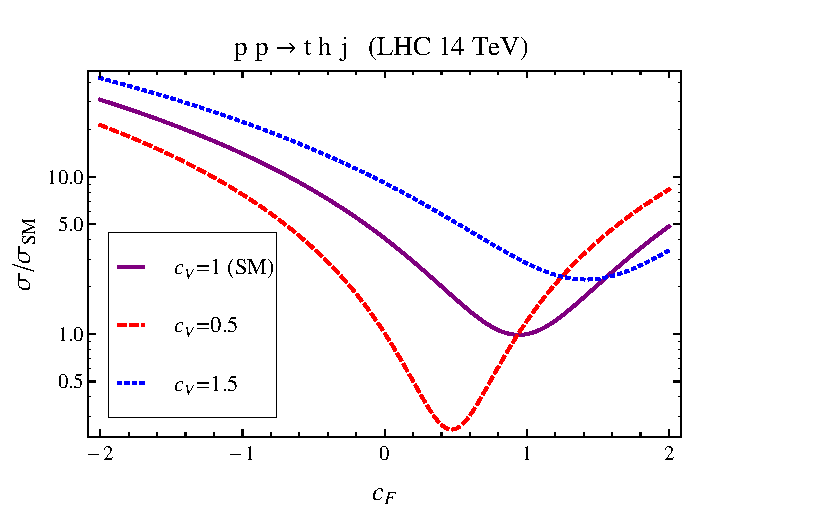
\includegraphics[scale=0.9]{thq_en}\\
\caption[Cross section for \tHq process as a function of $\kappa_t$]{Cross section for \tHq process as a function of $\kappa_t$, normalized to the SM, for three values of $\kappa_V$. In the plot $c_f$ refers to the Higgs-fermion coupling which is dominated by the H-t coupling and represented here by $\kappa_t$. Solid, dashed and dotted lines correspond to $c_V \to \kappa_V= 1, 0.5, 1.5$ respectively. Note that for the SM ($\kappa_V=\kappa_t=1$), the destructive effect of the interference is maximal.} 
\label{thq_en}
\end{figure}

\begin{figure}[h!]
\centering
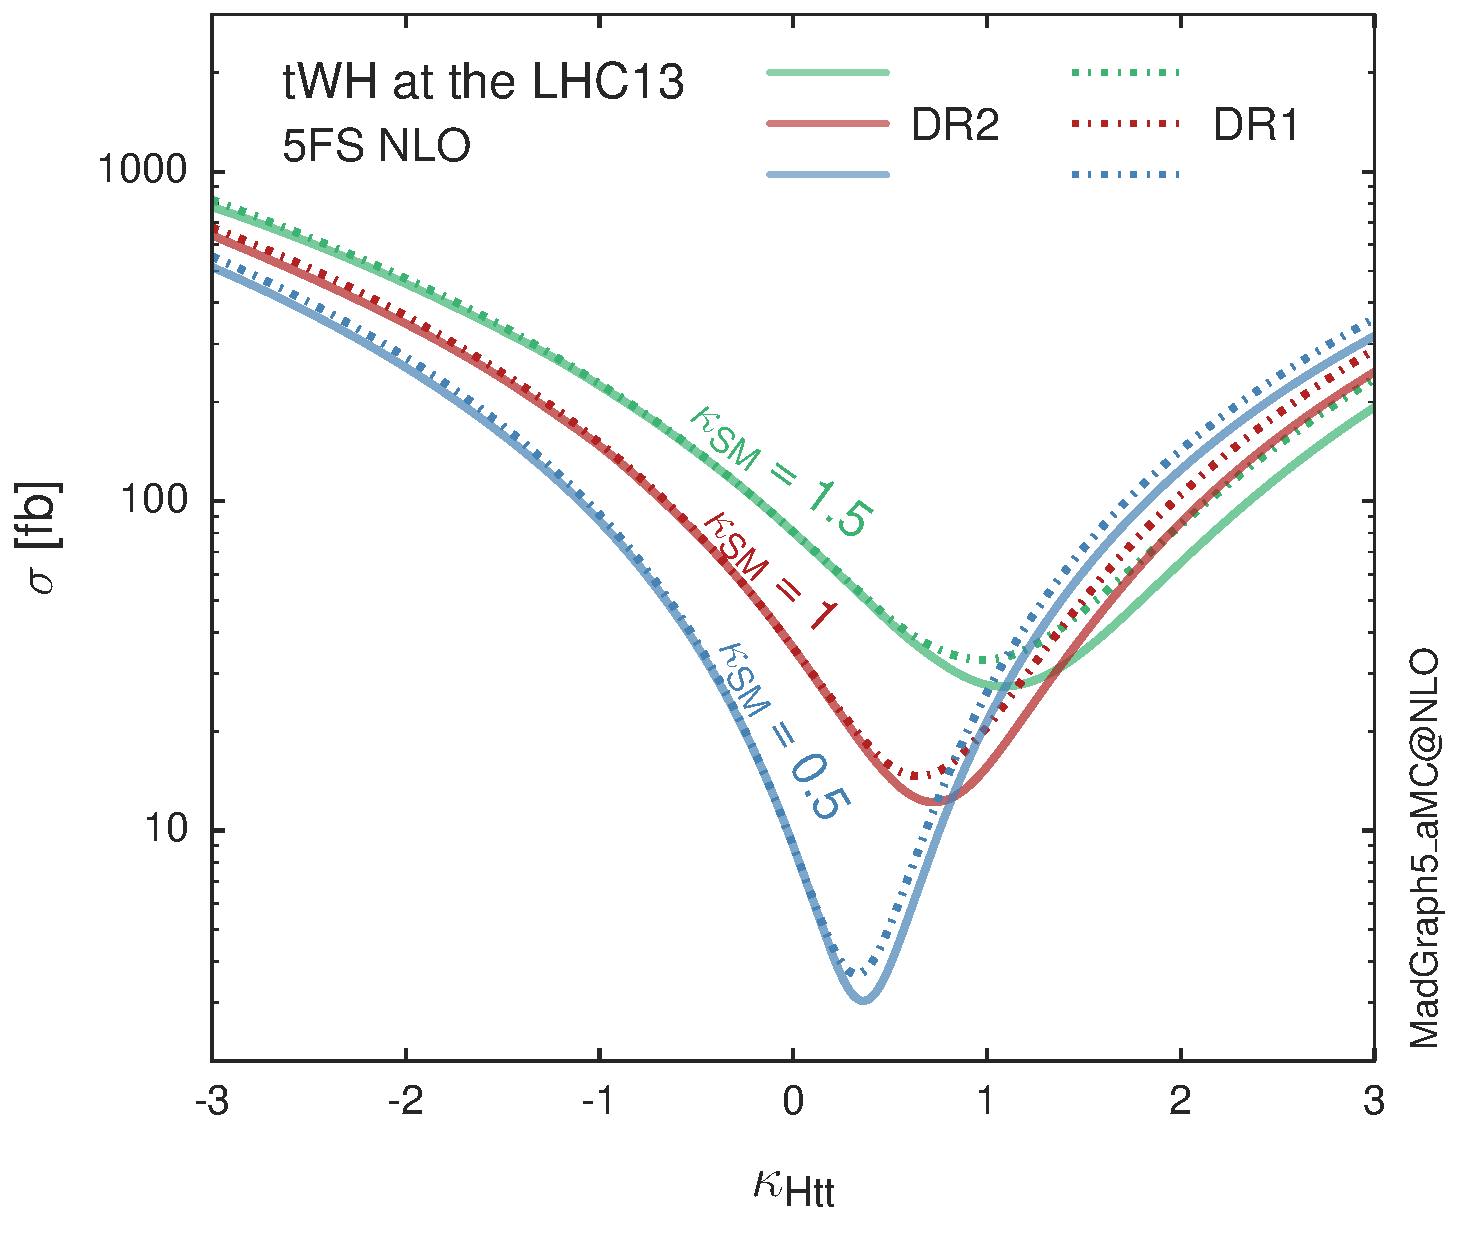
\includegraphics[scale=0.4]{thw_en}\\
\caption[Cross section for \tHW process as a function of $\kappa_{Htt}$]{Cross section for \tHW process as a function of $\kappa_{Htt}$, for three values of $\kappa_{SM}$ at $\sqrt{s}=13$ TeV. $\kappa_{Htt}^2=\sigma_{Htt}/\sigma_{Htt}^{SM}$ is a simple re-scaling of the SM Higgs interactions.} 
\label{thw_en}
\end{figure}

A similar analysis is valid for the W-associated channel but, in that case, the interference is more complicated since there are more than two contributions and an additional interference with the production of Higgs boson and a top pair process(\ttH). The calculations are made using the so-called Diagram Removal (DR) technique where interfering diagrams are removed (or added) from the calculations in order to evaluate the impact of the removed contributions. DR1 was defined to neglect \ttH interference while DR2 was defined to take \ttH interference into account\cite{demartin}. As shown in Figure \ref{thw_en}, the \tHW cross section is enhanced from about 15 fb (SM: $\kappa_{Htt}=1$) to about 150 fb ($\kappa_{Htt}=-1$). Differences between curves for DR1 and DR2 help to gauge the impact of the interference with \ttH.\\      
Results of the calculations of the \tHq and \tHW cross sections at $\sqrt{s}=13$ TeV can be found in Reference \cite{yellow} and a summary of the results is presented in Table \ref{tab:th_xsec_en}.
\begin{center}
\begin{table}[h]
\centering
\begin{tabular}{lcll}\hline
                                                            & $\sqrt{s}$ TeV   & $\kappa_t=1$                        & $\kappa_t=-1$                   \\\hline
\multirow{2}{*}{$\sigma^{LO}$(\tHq)(fb)\cite{farina}}       & 8                & $\approx 17.4$                 & $\approx 252.7$            \\
                                                            & 14               & $\approx 80.4$                 & $\approx 1042$             \\\hline
\multirow{2}{*}{$\sigma^{NLO}$(\tHq)(fb)\cite{farina}}      & 8                & $18.28^{+0.42}_{-0.38}$        & $233.8^{+4.6}_{-0.0}$      \\
                                                            & 14               & $88.2^{+1.7}_{-0.0}$           & $982.8^{+28}_{-0.0}$       \\\hline
$\sigma^{LO}$(\tHq)(fb) \cite{biswas2}                      & 14               & $\approx 71.8$                 & $\approx 893$              \\
$\sigma^{LO}$(\tHW)(fb) \cite{biswas2}                      & 14               & $\approx 16.0$                 & $\approx 139$              \\\hline
\multirow{3}{*}{$\sigma^{NLO}$(\tHq)(fb)\cite{yellow}}      & 8                & $18.69^{+8.62\%}_{-17.13\%}$   & -                          \\
                                                            & 13               & $74.25^{+7.48\%}_{-15.35\%}$   & $848^{+7.37\%}_{-13.70\%}$ \\
                                                            & 14               & $90.10^{+7.34\%}_{-15.13\%}$   & $1011^{+7.24\%}_{-13.39\%}$\\\hline
$\sigma^{LO}$(\tHW)(fb)\cite{demartin}                      & 13               & $15.77^{+15.91\%}_{-15.76\%}$  & -                          \\
$\sigma^{NLO} DR1$(\tHW)(fb)\cite{demartin}                 & 13               & $21.72^{+6.52\%}_{-5.24\%}$    & $\approx 150$              \\
$\sigma^{NLO} DR2$(\tHW)(fb)\cite{demartin}                 & 13               & $16.28^{+7.34\%}_{-15.13\%}$   & $\approx 150$              \\\hline
\end{tabular}
\caption[Predicted enhancement of the \tHq and \tHW cross sections at LHC]{Predicted enhancement of the \tHq and \tHW cross sections at LHC for $\kappa_V=1$ and $\kappa_t= \pm1$ at LO and NLO; the cross section enhancement of more that a factor of 10 is due to the flipping in the sign of the H-t coupling with respect to the SM one.}
\label{tab:th_xsec_en}
\end{table}
\end{center}

%% \begin{center}
%% \begin{table}[h]
%% \centering
%% \begin{tabular}{lcll}\hline
%%                                                             & $\sqrt{s}$ TeV   & $\kappa_t=1$                        & $\kappa_t=-1$                   \\\hline
%% \multirow{2}{*}{$\sigma^{LO}$(\tHq)(fb)\cite{farina}}       & 8                & $\approx 17.4$                 & $\approx 252.7$            \\
%%                                                             & 14               & $\approx 80.4$                 & $\approx 1042$             \\\hdashline
%% $\sigma^{LO}$(\tHq)(fb) \cite{biswas2}                      & 14               & $\approx 71.8$                 & $\approx 893$              \\
%% $\sigma^{LO}$(\tHW)(fb) \cite{biswas2}                      & 14               & $\approx 16.0$                 & $\approx 139$              \\%\hline
%% $\sigma^{LO}$(\tHW)(fb)\cite{demartin}                      & 13               & $15.77^{+15.91\%}_{-15.76\%}$  & -                          \\\hline
%% \multirow{2}{*}{$\sigma^{NLO}$(\tHq)(fb)\cite{farina}}      & 8                & $18.28^{+0.42}_{-0.38}$        & $233.8^{+4.6}_{-0.0}$      \\
%%                                                             & 14               & $88.2^{+1.7}_{-0.0}$           & $982.8^{+28}_{-0.0}$       \\\hdashline
%% \multirow{3}{*}{$\sigma^{NLO}$(\tHq)(fb)\cite{yellow}}      & 8                & $18.69^{+8.62\%}_{-17.13\%}$   & -                          \\
%%                                                             & 13               & $74.25^{+7.48\%}_{-15.35\%}$   & $848^{+7.37\%}_{-13.70\%}$ \\
%%                                                             & 14               & $90.10^{+7.34\%}_{-15.13\%}$   & $1011^{+7.24\%}_{-13.39\%}$\\\hdashline
%% $\sigma^{NLO} DR1$(\tHW)(fb)\cite{demartin}                 & 13               & $21.72^{+6.52\%}_{-5.24\%}$    & $\approx 150$              \\
%% $\sigma^{NLO} DR2$(\tHW)(fb)\cite{demartin}                 & 13               & $16.28^{+7.34\%}_{-15.13\%}$   & $\approx 150$              \\\hline
%% \end{tabular}
%% \caption[Predicted enhancement of the \tHq and \tHW cross sections at LHC]{Predicted enhancement of the \tHq and \tHW cross sections at LHC for $\kappa_V=1$ and $\kappa_t= \pm1$ at LO and NLO; the cross section enhancement of more that a factor of 10 is due to the flippling in the sign of the H-t coupling with respect to the SM one.}
%% \label{tab:th_xsec_en}
%% \end{table}
%% \end{center}

%______________________ cp phase ______________________
\section{CP-mixing in \tH processes}\label{sec:cp}

In addition to the sensitivity to sign of the H-t coupling, the \tHq and \tHW processes have been proposed as a tool to investigate the possibility of a H-t coupling that does not conserve CP\cite{maltoni2,demartin,ellis}. %Current experimental results are consistent with SM H-V and H-t couplings; however, negative H-t coupling is not excluded completely \cite{comb_ht_couplings}.\\

In this thesis, the sensitivity of \tH processes to CP-mixing is also studied on the basis of References \cite{maltoni2,demartin} using the effective field theory framework where a generic particle ($X_0$) of spin-0 and a general CP violating interaction with the top quark (Htt coupling), can couple to scalar and pseudo-scalar fermionic densities. The H-W interaction is assumed to be SM-like. The Lagrangian modeling the H-t interaction is given by

\beqn
\Lagr_0^t = -\bar\psi_t\left(c_{\alpha}\kappa_{Htt}g_{Htt}+i s_{\alpha}\kappa_{Att}g_{Att}\gamma_5 \right)\psi_t X_0,
\label{eq:l_cp}
\eeqn

\noindent where $\alpha$ is the CP-mixing phase, $c_\alpha\equiv\cos\alpha$ and $s_\alpha\equiv\sin\alpha$, $\kappa_{Htt}$ and $\kappa_{Att}$ are real dimensionless re-scaling parameters\footnote{analog to $\kappa_t$ and $\kappa_V$} used to parametrize the magnitude of the CP-violating and CP-conserving parts of the amplitude. The model defines $g_{Htt}=g_{Att}=m_t/v=y_t/\sqrt{2}$ with $v\sim 246$ GeV the Higgs vacuum expectation value. In this parametrization, three special cases can be recovered

\begin{itemize}
\item CP-even coupling $\to \alpha=0^o$  
\item CP-odd coupling $\to \alpha=90^o$
\item SM coupling $\to \alpha=0^o$ and $\kappa_{Htt}=1$  
\end{itemize}

The loop induced $X_0$ coupling to gluons can also be described in terms of the parametrization above, according to

\beqn
\Lagr_0^{g} = -\frac{1}{4}\left(c_{\alpha}\kappa_{Hgg}g_{Hgg}G_{\mu\nu}^aG^{a,\mu\nu}+s_{\alpha}\kappa_{Agg}g_{Agg}G_{\mu\nu}^a\widetilde G^{a,\mu\nu} \right)X_0.
\label{eq:l_Hglu}
\eeqn

\noindent where $g_{Hgg}=-\alpha_s/3\pi v$ and $g_{Agg}= \alpha_s/2\pi v$ and $G_{\mu\nu}$ is the gluon field strength tensors. Under the assumption that the top quark dominates the gluon-fusion process at LHC energies, $\kappa_{Hgg} \to \kappa_{Htt}$ and  $\kappa_{Agg} \to \kappa_{Att}$, so that the ratio between the gluon-gluon fusion cross section for $X_0$ and for the SM Higgs prediction can be written as     

\beqn
\frac{\sigma_{NLO}^{gg \to X_0} }{\sigma_{NLO,SM}^{gg \to H}}=  c^2_\alpha\kappa^2_{Htt}+s^2_\alpha \left( \kappa_{Att}\frac{g_{ Agg}}{g_{Hgg}} \right)^2.
\label{eq:GFrate}
\eeqn

If the re-scaling parameters are set to

\beqn
\kappa_{Htt}=1, \qquad \kappa_{Att}= \left|\frac{g_{Hgg}}{g_{Agg}}\right|=\frac{2}{3}.
\eeqn

\noindent the gluon-fusion SM cross section is reproduced for every value of the CP-mixing angle $\alpha$; therefore, by imposing that condition to the Lagrangian density \ref{eq:l_cp}, the CP-mixing angle is not constrained by current data. Figure \ref{xsec_alpha_thq} shows the NLO cross sections for t-channel $tX_0$(blue) and $t\bar{t}X_0$ (red) associated production processes as a function of the CP-mixing angle $\alpha$. $X_0$ is a generic spin-0 particle with top quark CP-violating coupling. Re-scaling factors $\kappa_{Htt}$ and  $\kappa_{Att}$ have been set to reproduce the SM gluon-fusion cross sections.   

\begin{figure}[h!]
\centering
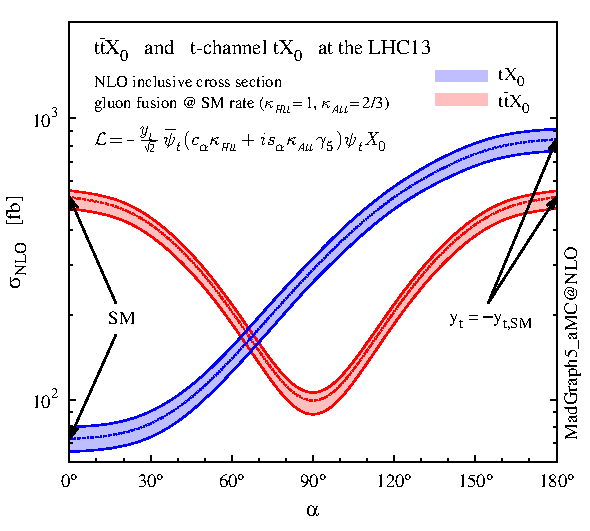
\includegraphics[scale=1.2]{xsec_alpha_thq}
\caption[NLO cross section for $tX_0$ and $t\bar{t}X_0$.]{NLO cross sections for t-channel $tX_0$(blue) and $t\bar{t}X_0$ (red) associated production processes as a function of the CP-mixing angle $\alpha$. $X_0$ is a generic spin-0 particle with top quark CP-violating coupling \cite{maltoni2}.} 
\label{xsec_alpha_thq}
\end{figure}

It is interesting to notice that the $tX_0$ cross section is enhanced, by a factor of about 10, when a continuous rotation in the scalar-pseudoscalar plane is applied; this enhancement is similar to the enhancement produced when the H-t coupling is flipped in sign with respect to the SM ($y_t=-y_{t,SM}$ in the plot), as showed in Section \ref{sec:thq}. In contrast, the degeneracy in the $t\bar{t}X_0$ cross section is still present given that it depends quadratically on the H-t coupling, but more interesting is to notice that $t\bar{t}X_0$ cross section is exceeded by $tX_0$ cross section after $\alpha\sim 60^o$.
\begin{figure}[h!]
\centering
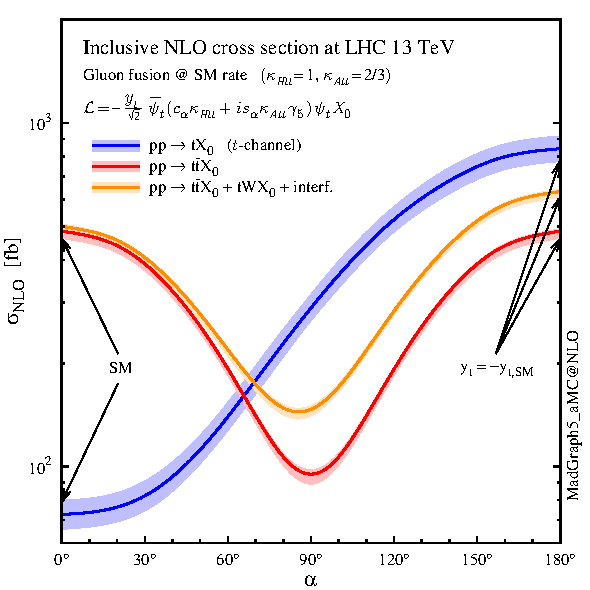
\includegraphics[scale=1.1]{xsec_alpha_thw}
\caption[NLO cross section for $tWX_0$, $t\bar{t}X_0$.]{NLO cross sections for t-channel $tX_0$(blue), $t\bar{t}X_0$ (red) associated production processes and combined $tWX_0 + t\bar{t}X_0$ (including interference) production as a function of the CP-mixing angle $\alpha$\cite{maltoni2}.} 
\label{xsec_alpha_thw}
\end{figure}

A similar parametrization can be used to investigate the \tHW process sensitivity to CP-violating H-t coupling. As said in \ref{sec:thq}, the interference in the W-associated channel is more complicated because there are more than two contributions and also there is interference with the \ttH production process.\\

Figure \ref{xsec_alpha_thw} shows the NLO cross sections for t-channel $tX_0$(blue), $t\bar{t}X_0$ (red) associated production and for the combined  $tWX_0 + t\bar{t}X_0 + interference$ (orange) as a function of the CP-mixing angle. It is clear that the effect of the interference in the combined case is the lifting of the degeneracy present in the $t\bar{t}X_0$ production. The constructive interference enhances the cross section from about 500 fb at SM ($\alpha=0$) to about 600 fb ($\alpha=180^o \to y_t=-y_{t,SM}$).  

An analysis combining \tHq and \tHW processes will be made in this thesis taking advantage of the sensitivity improvement.

